%\chapter{Vectors and Tensors}
\chapter{矢量和张量}
\label{chapter:vc}

出现在地球自由振荡所满足的方程中的物理量是矢量和张量,如位移、速度、应
变和应力;我们对这些方程的讨论以基本矢量和张量分析的知识为前提。
在本附录中我们针对使用的符号和一些基本结果做一个归纳。我们不提供任何证明,
因为我们的目的不是要取代如~Willmore (\citeyear{willmore59})
和 Marsden \& Hughes (\citeyear{marsden&hughes83})~等更系統性的数学讨论。
不同于这些作者,我们在这里采用基本的笛卡尔观点,
只有当我们在三维空间中的二维面上引入曲线坐标系统时,才会对协变和逆变加以区分。

%\section{Tensors as Multilinear Functionals}
\section{张量作为多重线性泛函}
\index{tensor|(}%

根据定义,张量是普通三维矢量空间上的一个多线性泛函。或者,我们
可以把一个~$q$~阶张量视为一线性算子,它作用于一个~$p$~阶张量,产生一个~$q-p$~阶
的张量。为了形象说明这两个概念的含义,更方便的是用一个比我们最终将采用(由吉布
斯发明)的更抽象的符号。

%\subsection{Vectors}
\subsection{矢量}
\index{vector|(}%

矢量是一个几何对象,通常被想象为一个箭头,有其大小和方向。
\index{vector!magnitude of}%
\index{vector!direction of}%
我们用粗体来表示矢量;矢量~$\bu$~的大小以~$\|\bu\|$~来表示。
\index{vector!norm}%
单位长度的矢量则在上方以一个帽子的符号来区分:$\|\bnh\|=1$。
\index{unit vector}%
\index{vector!unit}%
两个矢量~$\bu$~和~$\bv$~的标量积或{\em 点积\/}为 $\bu\cdot\bv=\|\bu\|\,\|\bv\|\cos\theta$, 
\index{scalar product}%
\index{dot product}%
其中~$\theta$~是两个矢量之间的锐角。请注意有~$\bu\cdot\bv=
\bv\cdot\bu$~和~$\|\bu\|=(\bu\cdot\bu)^{1/2}$。
两个矢量的矢量积或{\em 叉乘积\/}
\index{cross product}%
是一个大小为~$\|\bu\times\bv\|=\|\bu\|\,\|\bv\|\sin\theta$~ 的矢量,其方向由“右手法则”所定义。
一般有~$\bu\times\bv=-\bv\times\bu$~
和~$\bu\times\bu=\bzero$,其中~$\bzero$~是零矢量。
三个矢量的{\em 三重积\/}
\index{triple product}%
满足~$\bu\cdot(\bv\times\bw)
=\bw\cdot(\bu\times\bv)=\bv\cdot(\bw\times\bu)$,
而双重叉乘积的定义为~$\bu\times(\bv\times\bw)=(\bu\cdot\bw)\bv-
(\bu\cdot\bv)\bw$。

在笛卡尔座标系~$\bxh$、$\byh$、$\bzh$~中,一个矢量~$\bu$~的{\em 分量\/}为~$u_x=\bxh\cdot\bu$、$u_y=\byh\cdot\bu$、$u_z=\bzh\cdot\bu$。
$\bu$~可以用三个分量表示为~$\bu=u_x\bxh+u_y\byh+u_z\bzh$。
我们还可以采用更简洁的编号的坐标轴~ $\bxh_1$、$\bxh_2$、$\bxh_3$~来取代~$\bxh$、$\byh$、$\bzh$:

\eq \label{A.vecomp}
u_i=\bxh_i\cdot\bu,\qquad\bu=u_i\bxh_i.
\en

方程~(\ref{A.vecomp})~体现了求和约定的表达方式,
\index{summation convention}%
其中单一角标代表三个独立的方程,
而任何重复角标都意味着求和。两个矢量的点积以分量表示成~$\bu\cdot\bv=u_iv_i$
,而叉乘积~$\bw=\bu\times\bv$~则为~$w_i=\varepsilon_{ijk}u_jv_k$。
符号~$\varepsilon_{ijk}$~是~{\em Levi-Civit\`{a} 交替符号\/},
\index{Levi-Civit\`{a} alternating symbol}%
当~$\{i,j,k\}$~是~$\{1,2,3\}$~的偶数置换时,其值为~$1$,当~$\{i,j,k\}$~是~ $\{1,2,3\}$~的奇数置换时,其值为~$-1$,其余则为~$0$。该符号满足以下等式
\eqa \lefteqn{
\varepsilon_{ijk}\varepsilon_{lmn}=\delta_{il}\delta_{jm}\delta_{kn}
+\delta_{in}\delta_{jl}\delta_{km}+\delta_{im}\delta_{jn}\delta_{kl}}
\nonumber \\
&&\mbox{}
-\delta_{il}\delta_{jn}\delta_{km}
-\delta_{in}\delta_{jm}\delta_{kl}
-\delta_{im}\delta_{jl}\delta_{kn},
\ena
\eq
\varepsilon_{ijk}\varepsilon_{imn}=\delta_{jm}\delta_{kn}
-\delta_{jn}\delta_{km},
\en
\eq
\varepsilon_{ijk}\varepsilon_{ijn}=2\delta_{kn},
\qquad\varepsilon_{ijk}\varepsilon_{ijk}=6,
\en
其中 $\delta_{ij}$ 是{\em Kronecker 符号\/},
\index{Kronecker delta}%
\index{delta symbol}%
定义为当~$i=j$~时,其值为~$1$,当~$i\neq j$~时,其值为~$0$。在本附录中,我们大多都会使用角标符号;然而,在某些情况下,
例如在~\ref{A.sec.polcoord}节等处,我们发现使用“传统”的坐标轴~$\bxh$、$\byh$、 $\bzh$~会更方便。
\index{vector|)}%

%\subsection{Linear functionals}
\subsection{线性泛函}
\index{linear functional|(}%
\index{functional!linear|(}%

一个{\em 线性泛函\/}只是一个定义在三维矢量空间上的线性标量函数。
以~$f(\bu)$~表示由泛函~$f$~赋予矢量~$\bu$~的标量,我们要求
\eq \label{A.linfun}
f(a\bu+b\bv)=af(\bu)+bf(\bv).
\en
如同矢量一样,线性泛函的存在与任何笛卡尔坐标系无关,这个意义上说,线性泛函是一个~{\em 几何对象\/}。
利用Misner, Thorne \& Wheeler (\citeyear{misner&al73})~的花哨但物理上有说服力的类比,
我们将线性泛函~$f$~想象为一台有一个投币口的角子机。每当一个矢量被投入投币口,机器就会吐出一个标量:
\eq \label{A.linfun2}
\begin{array}{l}
f(\,\cdot\,)\rightarrow\mbox{scalar.} \\
\hspace{3.7 mm}\uparrow \\ \hspace{1.0 mm}
\raise.7ex\hbox{\scriptsize vector}
\end{array}
\en
如果投入矢量~$a\bu+b\bv$~的线性组合,机器就会按~(\ref{A.linfun})~生成标量的线性组合~$af(\bu)+bf(\bv)$。线性泛函的线性组合则显而易见地定义为
~$(af+bg)(\bu)=af(\bu)+bg(\bu)$。

对于任一线性泛函~$f$,都有一个唯一的矢量~$\bef$,它对所有矢量~$\bu$~都满足
\eq \label{A.linfun3}
f(\bu)=\bef\cdot\bu.
\en
我们称~$\bef$~代表~$f$。可以很容易证明,如果~$\bef$~代表~$f$,$\bg$~代表~$g$,则~ $a\bef+b\bg$~代表
~$af+bg$。任何如同~(\ref{A.linfun3})~一样保持矢量运算规则对应关系都被称为~{\em 同构\/}~的。
 \index{isomorphism}%
因为线性泛函和代表它们的矢量是代数不可区分的,
我们在下面可以也将会视它们为{\em 相同的\/}几何对象,只是从不同的角度来看。
将一个矢量~$\bef$~想象为具有一个线性投币口的角子机~(\ref{A.linfun2}),而不是一个箭头,初看起来像是奇怪的做法。然而,如我们接下来要讨论的,这种视角转换的优点是可以很容易推广到更高阶的张量。


\index{linear functional|)}%
\index{functional!linear|)}%

%\subsection{Multilinear functionals}
\subsection{多重线性泛函}
\index{multilinear functional|(}%
\index{functional!multilinear|(}%

一个~$q$~阶多重线性泛函,也被称为~$q$~{\em 阶张量\/},
\index{tensor!order of}%
是一个有~$q$~个线性投币口,输入矢量而输出标量的角子机:
\eq \label{A.tensor}
T(\,\underbrace{\cdot\,,\,\cdots\cdots\,,\,\cdot}
_{\mbox{\scriptsize {\it q} vector slots}}\,)\rightarrow\mbox{scalar}.
\en
将一组有序矢量~$\bu_1,\ldots,\bu_q$~依序投入这些投币口,
张量~$T$~会产生一个标量,表示为~$T(\bu_1,\ldots,\bu_q)$。
将一个矢量的线性组合投入到任一投币口,
我们会得到一个标量的线性组合:
\eq \label{A.tensor2}
T(\,\cdots,a\bu+b\bv,\cdots\,)=
aT(\,\cdots,\bu,\cdots\,)
+bT(\,\cdots,\bv,\cdots\,).
\en
阶数同为~$q$~的张量可分别与标量相乘并相加,形成线性组合,如~$aT+bP$。一个
一阶张量就是一个矢量,而一个零阶张量则默认为一个标量。

$q$~阶张量~$T$~和~$p$~阶张量~$P$~的外积或{\em 张量积\/}
\index{tensor product}%
是~$q+p$~阶的张量~$TP$ ,定义为
\eq \label{A.tensor3}
TP(\,\underbrace{\cdot\,,\,\cdots\cdots\,,\,\cdot}
_{\mbox{\scriptsize {\it q}+{\it p} slots}}\,)=
T(\,\underbrace{\cdot\,,\,\cdots\,,\,\cdot}
_{\mbox{\scriptsize {\it q} slots}}\,)
P(\,\underbrace{\cdot\,,\,\cdots,\,\cdot}
_{\mbox{\scriptsize{\it p} slots}}\,).
\en
由于张量中投币口的次序很重要,所以通常~$PT=TP$~{\em 并不\/}成立。两个
线性泛函的张量乘积~$fg$~被称为{\em 双并矢\/},
\index{dyad}%
而~$q$~个线性泛函的张量乘积~$f_1\cdots f_q$~被称为~$q$~{\em 阶多并矢\/}。
\index{polyad}%

一个二阶张量的{\em 迹\/}或{\em 缩并\/}为
\index{trace}%
\index{contraction}%
\index{tensor!trace of}%
\index{tensor!contraction of}%
\eq \label{A.trace}
{\rm tr}\,T=T(\bxh_i,\bxh_i),
\en
这里重复的角标仍然意味着求和。
更一般地,我们定义一个~$q$~阶张量的第~$r$~个和第~$s$~个投币口的缩并为
\eq \label{A.trace2}
\raise2.7ex\hbox{${\rm tr}_{rs}
T(\,\cdot\,,\,\cdots\cdots\,,\,\cdot\,)=$}
\begin{array}{l}
T(\,\cdots,\bxh_i,\cdots,\bxh_i,\cdots\,). \\
\hspace{11.0 mm}\uparrow\hspace{9.6 mm}\uparrow \\
\hspace{3.5 mm} \raise.7ex\hbox{\scriptsize {\it r}th slot}
\hspace{9.5 mm} \raise.7ex\hbox{\scriptsize {\it s}th slot}
\end{array}
\en
很容易证明,${\rm tr}\,T$~和~
${\rm tr}_{rs}T$~均与用来计算它们的笛卡尔坐标系~$\bxh_1$、$\bxh_2$、$\bxh_3$~无关。
缩并总是将张量的降低两阶,因而机器~${\rm tr}_{rs}T$~有~$q-2$~个投币口。

一个二阶张量的{\em 转置\/}是通过将两个投币口的顺序互换得到的:
\index{transpose}%
\index{tensor!transpose of}%
\eq \label{A.trans}
T^{\rm T}(\bu,\bv)=T(\bv,\bu).
\en
更一般地,我们将~$q$~阶张量的第~$r$~个和第~$s$~个投币口的转置表示为
\eq \label{A.trans2}
\begin{array}{l}
\Pi_{rs}T(\,\cdots,\bu,\cdots,\bv,\cdots\,) \\
\hspace{16.5 mm}\uparrow\hspace{8.3 mm}\uparrow \\
\hspace{9.0 mm} \raise.7ex\hbox{\scriptsize {\it r}th slot}
\hspace{8.2 mm} \raise.7ex\hbox{\scriptsize {\it s}th slot}
\end{array}
\raise2.7ex\hbox{$\!=$}
\begin{array}{l}
T(\,\cdots,\bv,\cdots,\bu,\cdots\,). \\
\hspace{11.0 mm}\uparrow\hspace{8.4 mm}\uparrow \\
\hspace{3.5 mm} \raise.7ex\hbox{\scriptsize {\it r}th slot}
\hspace{8.3 mm} \raise.7ex\hbox{\scriptsize {\it s}th slot}
\end{array}
\en
一个{\em 对称的\/}二阶张量满足~$S^{\rm T}=S$,而一个{\em 反对称的\/}张量则满足~$A^{\rm T}=-A$。
\index{symmetric tensor}%
\index{anti-symmetric tensor}%
\index{tensor!symmetric}%
\index{tensor!anti-symmetric}%
二阶{\em 单位张量\/}和三阶{\em 交替张量\/}的定义为:
\index{identity tensor}%
\index{alternating tensor}%
\index{tensor!identity}%
\index{tensor!alternating}%
\eq \label{A.ident}
I(\bu,\bv)=\bu\cdot\bv,\qquad
\Lambda(\bu,\bv,\bw)=\bu\cdot(\bv\times\bw).
\en
这两个张量对于每个投币口都分别是对称的和反对称的,即~
$I^{\rm T}=I$, 而~$\Lambda=-\Pi_{12}\Lambda
=-\Pi_{13}\Lambda=-\Pi_{23}\Lambda$。
\index{multilinear functional|)}%
\index{functional!multilinear|)}%

%\subsection{Components}
\subsection{分量}
\index{component!of a tensor|(}%
\index{tensor!components of|(}%

一个矢量~$\bef$~的三个分量~$f_i=\bxh_i\cdot\bef$~由
相应的线性泛函~$f$~以~$f_i=f(\bxh_i)$~给定。 一个~$q$~阶张量的~$3^q$~ 个分量由类似的方式所定义:
\eq \label{A.comps}
T_{i_1\cdots\,i_q}=T(\bxh_{i_1},
\ldots,\bxh_{i_q}).
\en
正如每个矢量~$\bef=f_i\bxh_i$~完全由其在任一笛卡尔坐标系的分量所决定,每个
张量也是如此;事实上,
\eq \label{A.comps2}
T=T_{i_1\cdots\,i_q}\bxh_{i_1}\!\cdots\bxh_{i_q}.
\en
(\ref{A.comps2})~式两边的机器对任一有序的矢量序列 $T(\bu_1,\ldots,\bu_q)=T_{i_1\cdots\,i_q}
\bxh_{i_1}\!\cdots\bxh_{i_q}(\bu_1,\ldots,\bu_q)$~赋予相同的标量。
这~$3^q$~个多并矢~$\bxh_{i_1}\!\cdots\bxh_{i_q}$~构成了一个所有~$q$~ 阶张量空间的基。
例如,一个二阶张量可以用九个双并矢~$\bxh_i\bxh_j$~ 写为~$T=T_{ij}\bxh_i\bxh_j$~的形式。

张量运算可以用分量来进行;一个~$q$~阶张量与一个~$p$~阶张量的外
积为
\eq
(TP)_{i_1\cdots\,i_qj_1\cdots\,j_p}=T_{i_1\cdots\,i_q}
P_{j_1\cdots\,j_p},
\en
二阶张量的迹为
\eq
{\rm tr}\,T=T_{ii}.
\en
更一般地,对于一个~$q$~阶张量有
\eq
\raise2.7ex\hbox{$({\rm tr}_{rs}
T)_{i_1\cdots\,i_{q-2}}=$}
\begin{array}{l}
T_{i_1\cdots\,j\,\cdots\,j\,\cdots\,i_{q-2}}. \\
\hspace{7.4 mm}\uparrow\hspace{2.7 mm}\uparrow \\
\hspace{-2.5 mm} \raise.7ex\hbox{\scriptsize {\it r}th index}
\hspace{2.8 mm} \raise.7ex\hbox{\scriptsize {\it s}th index}
\end{array}
\en
转置张量~$T^{\rm T}$~和~$\Pi_{rs}T$~的角标有所置换:$T^{\rm T}_{ij}=T_{ji}$~和~ $(\Pi_{rs}T)_{\cdots j\cdots k\cdots}=
T_{\cdots k\cdots j\cdots}$,其中后一个表达式中省略号表示未受影响的角标。
对称的二阶张量~$S$~的分量满足~$S_{ij}=S_{ji}$,而反对称张量~$A$~的分量满足~ $A_{ij}=-A_{ji}$ 。

一个~$q$~阶张量在一个新的带撇号的笛卡尔坐标系~$\bxh_1^{\prime}$、$\bxh_2^{\prime}$、
$\bxh_3^{\prime}$~中的~$3^q$~个分量~$T_{i_1\cdots\,i_q}^{\prime}$
\vspace{-0.8 mm}与其在原来不带撇号坐标系~$\bxh_1$、$\bxh_2$、$\bxh_3$~中的分量~$T_{j_1\cdots\,j_q}$~之间的关系为
\eqa \label{A.comprel} \lefteqn{
T_{i_1\cdots\,i_q}^{\prime}=T(\bxh_{i_1}^{\prime},
\ldots,\bxh_{i_q}^{\prime})} \nonumber \\
&&\mbox{}\hspace{3.0 mm}=T((\bxh_{i_1}^{\prime}\cdot\bxh_{j_1})\bxh_{j_1},
\ldots,(\bxh_{i_q}^{\prime}\cdot\bxh_{j_q})\bxh_{j_q}) \nonumber \\
&&\mbox{}\hspace{3.0 mm}=(\bxh_{i_1}^{\prime}\cdot\bxh_{j_1})
\cdots(\bxh_{i_q}^{\prime}\cdot\bxh_{j_q})
T(\bxh_{j_1},\ldots,\bxh_{j_q}) \nonumber \\
&&\mbox{}\hspace{3.0 mm}=(\bxh_{i_1}^{\prime}\cdot\bxh_{j_1})
\cdots(\bxh_{i_q}^{\prime}\cdot\bxh_{j_q})T_{j_1\cdots\,j_q}.
\ena
坐标轴刚性旋转下分量之间的变换关系~(\ref{A.comprel})~是很多张量入门
讨论的起点;这里具有线性投币口角子机的处理方式与之完全等效,却具有一种更强的几何意味。


\index{component!of a tensor|)}%
\index{tensor!components of|)}%

%\subsection{Isotropic tensors}
\subsection{各向同性张量}
\index{tensor!isotropic|(}%
\index{isotropic tensor|(}%
\label{A.sec.iso}

(\ref{A.ident})~中定义的二阶单位张量和三阶交替张量的分量分别为克罗内克符号
和 Levi-Civit\`{a} 交替符号:
\index{Levi-Civit\`{a} alternating symbol}%
\index{Kronecker delta}%
\index{delta symbol}%
\eq
I_{ij}=\delta_{ij},\qquad \Lambda_{ijk}=\varepsilon_{ijk}.
\en
像~$I$~和~$\Lambda$~这样在所有右手坐标系~$\bxh_1$、$\bxh_2$、 $\bxh_3$~中都具有相同分量的张量被称做是{\em 各向同性的\/}。
各向同性的一阶张量只有唯一的零矢量。
每个各向同性的二阶张量都是单位张量~$I$~的倍数,
而每个各向同性的三阶张量都是交替张量~$\Lambda$~的倍数。
更高阶的各向同性张量是角标置换后的~$I$~或~$\Lambda$~的乘积的线性组合。
例如,最一般的四阶各向同性张量的形式为~$aII+b\hspace{0.2 mm}\Pi_{23}(II)+c\hspace{0.2 mm}\Pi_{24}(II)$,
其中~$a$、$b$~和~$c$~为标量。
我们将上述一到四阶张量的结果以分量形式归纳在表~A.1~中。
\begin{table}[h]
\centering
\begin{tabular}{|c|l|} \hline
& \\
阶数 & 各向同性矩阵的形式
& \\ \hline
& \\
$0$ & 所有标量 \\
$1$ & 仅有零矢量 \\
$2$ & $a\delta_{ij}$ \\
$3$ & $a\varepsilon_{ijk}$ \\
$4$ & $a\delta_{ij}\delta_{kl}+b\delta_{ik}\delta_{jl}
+c\delta_{il}\delta_{jk}$ \\
& \\ \hline
\end{tabular}
\caption[isoten]{
最一般的一到四阶各向同性张量。严格说来,三阶交替张量是一个手性的而不是完全的各向同性张量,因为其分量在从右手笛卡尔坐标系变换到左手坐标系时会改变符号。除了零张量之外,没有任何阶数~$q$~为奇数的张量是完全各向同性的。}
\end{table}
\index{tensor!isotropic|)}%
\index{isotropic tensor|)}%

%\subsection{Wedge operator}
\subsection{楔形算子}
\index{wedge operator|(}%
\index{operator!wedge|(}%
\label{sec.A.1.6}

楔形算子~$\wedge$~作用于一个二阶张量~$T$,产生的矢量~$\wedge T$~为
\eq \label{A.wedge}
\wedge T={\rm tr}_{23}{\rm tr}_{35}(\Lambda T).
\en
用角标符号可以将其写为更容易理解的形式:
\eq \label{A.wedge2}
(\wedge T)_i=\varepsilon_{ijk}T_{jk}.
\en
将楔形算子作用于一个双并矢,可以得到双并矢中两个矢量的叉乘积:
\eq
\wedge(\bef\bg)
=\bef\times\bg.
\en
\index{wedge operator|)}%
\index{operator!wedge|)}%
事实上,上式提供了使用该名称的动机,因为叉乘积~$\bef\times\bg$~的另一个写法是~$\bef\wedge\bg$。
当且仅当被作用的张量为对称($T^{\rm T}=T$)时,
楔形算子作用所得到的矢量为~0,即~$\wedge T=\bzero$。

%\section{Tensors as Linear Operators}
\section{张量作为线性算子}
\index{linear operator|(}%
\index{operator!linear|(}%

我们也可以把一个~$q$~阶张量看作是有单一线性投币口的机器,当输入~$p$~阶
张量时它输出~$q-p$~阶张量。从物理的观点,张量作为线性算子的
这种几何图像常常是更自然的。我们首先考虑~$q=2$~阶张量,且~$p=q-p=1$。
%\subsection{Second-order tensors}
\subsection{二阶张量}
\index{second-order tensor|(}%
\index{tensor!second-order|(}%

一个矢量取值的{\em 线性算子\/}~$\psi$~是一个如下形式的有单一投币口的机器
\index{linear operator}%
\index{operator!linear}%
\eq \label{A.linop}
\begin{array}{l}
\psi(\,\cdot\,)\rightarrow\mbox{vector.} \\
\hspace{3.7 mm}\uparrow \\ \hspace{1.0 mm}
\raise.7ex\hbox{\scriptsize vector}
\end{array}
\en
投入一个矢量的线性组合会产生一个输出矢量的线性组合:
\eq \label{A.linop2}
\psi(a\bu+b\bv)=a\psi(\bu)+b\psi(\bv).
\en
线性算子的线性组合可以用一个已经熟悉的方式定义: $(a\psi+b\chi)(\bu)=a\psi(\bu)+b\chi(\bu)$。每个线性算子~$\psi$~ 按以下对应关系生成一个唯一的二阶张量~$T_{\psi}$:
\eq \label{A.linop3}
T_{\psi}(\bu,\bv)=\bu\cdot\psi(\bv).
\en
该对应关系是同构的,因为
\index{isomorphism}%
$T_{a\psi+b\chi}=aT_{\psi}+bT_{\chi}$.
单位张量~$I$~是由{\em 单位算子\/}所产生,
\index{identity operator}%
\index{operator!identity}%
它只是将输入矢量原封不动地输出,即~$\psi(\bu)=\bu$。当然这也是其名称的来源。

线性算子的{\em 转置\/}~$\psi^{\rm T}$~定义为
\index{linear operator!transpose of}%
\index{operator!linear!transpose of}%
\eq \label{A.linop4}
\psi^{\rm T}(\bu)\cdot\bv=\bu\cdot\psi(\bv).
\en
很显然~$(\psi^{\rm T})^{\rm T}=\psi$。一个算子的转置和由它所生成的张量的转置是一样的,
因为~$T_{\psi^{\rm T}}=(T_{\psi})^{\rm T}$。一个{\em 对称\/}线性算子满足~ $\psi^{\rm T}=\psi$,
\index{linear operator!symmetric}%
而一个反对称算子
满足~$\psi^{\rm T}=-\psi$。而两个算子的{\em 乘积\/}的定义是
\index{linear operator!product of}%
\eq \label{A.linop5}
\psi\chi(\bu)=\psi(\chi(\bu)).
\en
惯例上是右边的算子先作用,也就是说,我们把~$\chi$~的输出投入~ $\psi$。算子的乘积一般是不互易的:即~
$\psi\chi\neq\chi\psi$。在转置时算子的顺序对换:即~$(\psi\chi)^{\rm T}=\chi^{\rm T}\psi^{\rm T}$。由~$T_{\psi\chi}$~生成的张量~$T_{\psi\chi}$~是什么?不是~ $T_{\psi}T_{\chi}$,因为这是一个四阶张量。事实上,它应该是
\eq \label{A.linop6}
T_{\psi\chi}={\rm tr}_{23}(T_{\psi}T_{\chi}).
\en
一旦建立了这些结果,我们便可以开始对二阶张量和矢量线性算子不做区别,就像我们对矢量和线性函数不做区别一样。在以下的部分,我们将不再区分~$\psi$~和~ $T_{\psi}$;用相同的符号来表示一个线性算子和它所生成的张量。

%\subsection{Components of a second-order tensor}
\subsection{二阶张量的分量}
简单来讲,一个线性算子~$T$~的{\em 分量\/}~$T_{ij}$~就是其对应张量的分量。
\index{second-order tensor!components of}%
\index{tensor!second-order!components of}%
线性关系~$\bu=T(\bv)$~可以用角标符号写为熟悉的形式
\eq \label{A.uiTijvj}
u_i=T_{ij}v_j.
\en
将分量~$T_{ij}$~排列成一个~$3\times 3$~矩阵,我们可以将方程~(\ref{A.uiTijvj})~ 明确地写为
\eq \label{A.ueqTv}
\left(\begin{array}{c}
u_1 \\ u_2 \\ u_3 \end{array}\right)=
\left(\begin{array}{ccc}
T_{11} & T_{12} & T_{13} \\
T_{21} & T_{22} & T_{23} \\
T_{31} & T_{32} & T_{33} \\
\end{array}\right)
\left(\begin{array}{c}
v_1 \\ v_2 \\ v_3 \end{array}\right).
\en
(\ref{A.ueqTv})~这一结果使我们可以通过矩阵相乘来计算线性算子~$T=T_{ij}\bxh_i\bxh_j$~在矢量~$\bv=v_j\bxh_j$~处的值。

一个线性算子作用于笛卡尔单位矢量 $\bxh_1,\bxh_2,\bxh_3$ 的效果可以用张量的分量表示为
\eq \label{A.perverse}
T(\bxh_i)=T_{ji}\bxh_j.
\en
$T_{ij}$~在~(\ref{A.uiTijvj})~中和~$T_{ji}$~在~(\ref{A.perverse})~中的 的出现是一个无法避免的特性,
Halmos (\citeyear{halmos58})~称之为“任性的角标。

%\subsection{Determinant and inverse}
\subsection{行列式和逆}
\index{determinant|(}%
\index{inverse of a tensor|(}%
\index{tensor!inverse of|(}%

一个线性算子~$T$~的{\em 行列式\/}是其在任一笛卡尔坐标系中分量的矩阵的行列式,其定义为
\eq \label{A.detdefn}
{\rm det}\,T=\sixth\eps_{ijk}\eps_{lmn}
T_{il}T_{jm}T_{kn}.
\en

无论使用什么坐标系~$\bxh_1$、$\bxh_2$、$\bxh_3$,(\ref{A.detdefn})~都会得到同样的结果;这确保在~${\rm det}\,T$~是一个几何对象。算子乘积的行列式是它们行列式的乘积:
${\rm det}\,TP=({\rm det}\,T)({\rm det}\,P)$。一个非奇异算子~$T$~的行列式为非零:即${\rm det}\,T\neq 0$。
每一个这种算子都有一个唯一的{\em 逆\/}~$T^{-1}$,满足当且仅当~$\bu=T(\bv)$~时, $\bv=T^{-1}(\bu)$;换句话说,$T^{-1}T=TT^{-1}=I$。若两个线性算子~$T$~和~$P$~均 为可逆的,则它们的乘积亦为可逆,且~$(TP)^{-1}=P^{-1}T^{-1}$。
一个算子的转置的逆就是其逆的转置:$(T^{\rm T})^{-1}
=(T^{-1})^{\rm T}$。有鉴于此,我们将使用浓缩的符号~$T^{-{\rm T}}$。显然有~${\rm det}\,T^{\rm T}={\rm det}\,T$~
以及~${\rm det}\,T^{-1}=({\rm det}\,T)^{-1}$。逆算子~$T^{-1}$~的分量~$T_{ij}^{-1}$ 可以用~$T$~的行列式~${\rm det}\,T$~及其分量~$T_{ij}$~表示为:
\eq \label{A.Cramrule}
T_{ij}^{-1}=\half({\rm det}\,T)^{-1}\varepsilon_{imn}
\varepsilon_{jkl}T_{km}T_{ln}.
\en
(\ref{A.Cramrule})~式是简洁的角标形式的求解三元联立线性方程组著名算法:{\em 克莱姆法则\/}。
\index{Cramer's rule}%
\index{determinant|)}%
\index{inverse of a tensor|)}%
\index{tensor!inverse of|)}%
\index{second-order tensor|)}%
\index{tensor!second-order|)}%

%\subsection{Higher-order tensors}
\subsection{高阶张量}
\index{higher-order tensor|(}%
\index{tensor!higher-order|(}%

$q>2$~阶的张量或多重线性泛函~$\Gamma$~与单投币口的线性算子之间也有同构关系
\index{isomorphism}%
\eq \label{A.tenop}
\begin{array}{l}
\Gamma(\,\cdot\,)\rightarrow\mbox{tensor of order $q-p$.} \\
\hspace{4.1 mm}\uparrow \\ \hspace{1.4 mm}
\raise.7ex\hbox{\scriptsize tensor of order {\it p}}
\end{array}
\en
与二阶张量的对应关系一样,保持投币口的整齐顺序是很重要的;与~(\ref{A.uiTijvj})~式类似,张量~$T=\Gamma(\eps)$~的分量为
\eq \label{A.ReqTS}
T_{i_1\cdots\,i_{q-p}}=\Gamma_{i_1\cdots\,i_{q-p}j_1\cdots\,j_p}
\eps_{\textcolor{red}{j_1}\cdots\,j_p}.
\en
任何线性本构关系都具有~(\ref{A.ReqTS})~的形式。例如,在经典弹性介质中
联系应力~$T_{ij}$~和应变~$\eps_{kl}$~的胡克“定律”为~ $T_{ij}=\Gamma_{ijkl}\eps_{kl}$。
在这一特例中,四阶弹性张量的对称性~$\Gamma_{ijkl}=\Gamma_{jikl}=\Gamma_{ijlk}=\Gamma_{klij}$~使我们能够变换角标的顺序。在更一般情况下,这样做是不行的。
\index{higher-order tensor|)}%
\index{tensor!higher-order|)}%
\index{linear operator|)}%
\index{operator!linear|)}%

%\section{Gibbs Notation}
\section{吉布斯符号}
\index{Gibbs notation|(}%
\index{index notation|(}%
\label{A.sec.Gibbs}

吉布斯~(\citeyear{gibbs01})~所发展的不变符号体系,为处理矢量和二阶张量提供了一种非常
方便的手段。我们在此做一个概括的介绍,本书自始至终都使用了这种符号。
矢量和张量都以粗体字母表示。
一般来说,矢量用小写字母,而张量用大写字母。(但若此惯例与公认的地震学传统相冲突时,我们会忽略它;例如,我们以小写的~$\beps$~来表示无穷小应变张量。)
张量~$\bT$~的转置写成~$\bT^{\rm T}$,逆
写成~$\bT^{-1}$,而转置的逆写成~$\bT^{-{\rm T}}$。两个张量~$\bT$~和~$\bP$~的外积用~ $\bT\bP$~表示,中间没有乘积的符号。因此,由矢量~$\bef_1,\ldots,\bef_q$~形成的~$q$~ 阶多并矢表示成~$\bef_1\!\cdots\bef_q$;
我们在说明~$3^q$~个多并矢~$\bxh_{i_1}\!\cdots\bxh_{i_q}$~构成~ $q$~阶张量空间的基时已经使用了这一写法。
双重线性泛函~$\bT$~赋予矢量~$\bu$~和~$\bv$~的标量用~$\bu\cdot\bT\cdot\bv$~表示,
而线性算子~$\bT$~赋予~$\bu$~的矢量则用~$\bT\cdot\bu$~表示。
转置算子~$\bT^{\rm T}$~赋予~$\bu$~的矢量表示为~$\bT^{\rm T}\cdot\bu
=\bu\cdot\bT$。最后,两个张量~$\bT$~和~$\bP$~的算子乘积表示成~$\bT\cdot\bP={\rm tr}_{23}(\bT\bP)$。

这个符号的优美之处在于,“点”具有“四重含义”。首先,在两个矢量~$\bu$~和~$\bv$~之间,
它是普通的点积~$\bu\cdot\bv$;将一个矢量~$\bu$~在右边点乘张量~$\bT$,得到相应的线
性算子~$\bT\cdot\bu$~的值,而将同一个矢量在左边点乘~$\bT$ ,则得到转置线性算子~ $\bu\cdot\bT=\bT^{\rm T}\cdot\bu$~的值。
最后,两个张量~$\bT$~和~$\bP$~之间的“点”表示算子乘积~ $\bT\cdot\bP$。这样一个多用途的点积使我们能够在某些公式中随意去除或添加括号,
如~$\bu\cdot\bT\cdot\bv=\bu\cdot(\bT\cdot\bv)=(\bu\cdot\bT)\cdot\bv$。
我们立刻能够看出,算子乘积~$(\bu\bef)\cdot(\bg\bv)$~
是加权的双并矢~$\bu(\bef\cdot\bg)\bv$。一个非奇异张量的逆满足~ $\bT^{-1}\cdot\bT=\bT\cdot\bT^{-1}=\bI$,其中~$\bI$~ 为单位张量。算子点积的转置和逆则分别由~$(\bT\cdot\bP)^{\rm T}=\bP^{\rm T}\cdot\bT^{\rm T}$~和~
$(\bT\cdot\bP)^{-1}=\bP^{-1}\cdot\bT^{-1}$~给定。

每一个“点”都表示相邻投币口的缩并,因此很容易将一个以吉布斯符号表示的
不变表达式转化为角标符号,反之亦然。
标量~$\bu\cdot\bT\cdot\bv$~为~$u_iT_{ij}v_j$,而矢量~$\bT\cdot\bu$~
和~$\bu\cdot\bT=\bT^{\rm T}\cdot\bu$~的分量则分别为~$T_{ij}u_j$~和~$u_jT_{ji}=T^{\rm T}_{ij}u_j$。
\index{double dot product}%
我们也使用双点积来表示两个相邻角标的缩并:
\eq \label{A.dubdot}
\bT\!:\!\bP={\rm tr}(\bT^{\rm T}\cdot\bP)
={\rm tr}(\bT\cdot\bP^{\rm T})
=T_{ij}P_{ij}.
\en
我们在本书中很少会有需要定义二阶张量的范数的场合;
如果有的话,我们始终是指~Frobenius~即普通的欧式范数~$\|\bT\|=(\bT\!:\!\bT)^{1/2}$。
\index{tensor!norm of}%
\index{norm!tensor}%

矢量和双并矢的{\em 叉乘积\/}也可以无需括号的方式来定义:
\index{cross product}%
\eq \label{A.cross}
\bu\times\bv\bw=(\bu\times\bv)\bw,\qquad
\bv\bw\times\bu=\bv(\bw\times\bu).
\en
要得到矢量与一般二阶张量的叉乘积,只需展开~$\bu=u_k\bxh_k$~和~ $\bT=T_{ij}\bxh_i\bxh_j$
并利用其线性性质。由此我们发现
\eq
\bP=\bu\times\bT,\qquad\bM=\bT\times\bu
\en
的分量可以表示为
\eq
P_{ij}=\eps_{ikl}u_kT_{lj},\qquad M_{ij}=\eps_{jlk}T_{il}u_k.
\en
对矢量乘张量或张量乘矢量的叉乘积进行转置的结果为~
$(\bu\times\bT)^{\rm T}=-\bT^{\rm T}\times\bu$~和~
$(\bT\times\bu)^{\rm T}=-\bu\times\bT^{\rm T}$。两个更高阶张量的单点积或叉乘积可以用类似的方式来理解;在任何诸如~$\bT\cdot\bP$~或~$\bT\times\bP$~的组合中,都是由左边张量的最后一个投币口与右边张量的第一个投币口做縮併或叉乘。

在上述完全的吉布斯符号之上,我们做两个小修改。首先,我们对双点积稍加推广,以~ $\bT=\bGamma\!:\!\beps$~和~$\beps\!:\!
\bGamma\!:\!\beps$~分别表示~$T_{ij}=\Gamma_{ijkl}\eps_{kl}$~和~ $\eps_{ij}\Gamma_{ijkl}\eps_{kl}$。
其次,我们利用“三个点”来表示两个高阶张量{\em 所有\/}角标的依序缩并:
\index{triple dot product}%
\eq \label{A.tdotdef}
\bT\tdot\bP={\rm tr}_{12}{\rm tr}_{13}\cdots{\rm tr}_{1q}
{\rm tr}_{1\,q+1}(\bT\bP)
=T_{i_1\cdots\,i_q}P_{i_1\cdots\,i_q}.
\en
一个张量的~$3^q$~个分量可以用该不变符号表示为~$T_{i_1\cdots i_q}
=(\bxh_{i_1}\cdots\bxh_{i_q})\tdot\bT$。
\index{tensor!norm of}%
\index{norm!tensor}%
$\bT$~的欧氏范数为~$\|\bT\|=(\bT\tdot\bT)^{1/2}$。

尽管有上述扩展,许多涉及更高阶张量的更复杂的运算还是无法用吉布斯符号书写成优雅的形式。例如,分量为~$u_jT_{ijk}$~和~$P_{jk}M_{ijkl}$~的张量的表达式分别为~$\bu\cdot(\Pi_{12}\bT)$~和~$\bP\!:\!(\Pi_{23}\Pi_{12}\bM)$。
面对这种棘手的表达式,大多数人会直接把它们转换成角标符号来理解其含义。在本书中,我们尽可能多地使用吉布斯符号;然而,只要有助于理解,我们也会毫不犹豫地使用角标符号。
\index{Gibbs notation|)}%
\index{index notation|)}%
\index{tensor|)}%

%\section{Cartesian and Polar Decomposition}
\section{笛卡尔和极坐标分解}
\index{polar decomposition|(}%
\index{Cartesian decomposition|(}%
\index{decomposition!polar|(}%
\index{decomposition!Cartesian|(}%

每个{\em 对称\/}张量~$\bS=\bS^{\rm T}$~
\index{symmetric tensor}%
\index{tensor!symmetric}%
都有三个实数{\em 本征值\/}~$\lambda_1$、$\lambda_2$、$\lambda_3$~
\index{eigenvalue}%
\index{tensor!eigenvalue of}%
和与其对应的三个相互垂直的单位{\em 本征矢量/}~$\betah_1$、$\betah_2$、$\betah_3$,
\index{eigenvector}%
\index{tensor!eigenvector of}%
满足以下条件
\eq \label{A.eigen}
\bS\cdot\betah_1=\lambda_1\betah_1,\qquad
\bS\cdot\betah_2=\lambda_2\betah_2,\qquad
\bS\cdot\betah_3=\lambda_3\betah_3.
\en
我们可以将该张量以三个双并矢之和写为{\em 对角形式\/}:
\index{diagonal form}%
\index{tensor!diagonal form of}%
\eq
\bS=\lambda_1\betah_1\betah_1+\lambda_2
\betah_2\betah_2+\lambda_3\betah_3\betah_3.
\en
由相对于基~$\betah_1$、$\betah_2$、$\betah_3$~的分量组成的矩阵的当然就是
\eq
\left(\begin{array}{ccc}
S_{11} & S_{12} & S_{13} \\
S_{21} & S_{22} & S_{23} \\
S_{31} & S_{32} & S_{33} \end{array}\right)
=\left(\begin{array}{ccc}
\lambda_1 & 0 & 0 \\
0 & \lambda_2 & 0 \\
0 & 0 & \lambda_3 \end{array}\right).
\en
一个{\em 正定\/}对称张量对每个矢量~$\bu$~都满足~$\bu\cdot\bS\cdot\bu>0$。
\index{positive definite tensor}%
\index{tensor!positive definite}%
一个对称张量为正定的条件是:其所有本征值均为正,即~$\lambda_1>0$、 $\lambda_2>0$、$\lambda_3>0$。
但是如果~$\bu\cdot\bS\cdot\bu\geq 0$,则~ $\bS$~被称为是正半定的;在这种情况下,其本征值只是非负的:即~$\lambda_1\geq 0$、 $\lambda_2\geq0$、$\lambda_3\geq0$。每个正定对称张量都有唯一的正定{\em 平方根\/},满足关系~$\bS^{1/2}\cdot\bS^{1/2}=\bS$。
\index{tensor!square root of}%
\index{square root of a tensor}%
要得到~$\bS^{1/2}$,我们将~$\bS$~对角化,并取本征值的平方根:
\eq
\bS^{1/2}=\sqrt{\lambda_1}\betah_1\betah_1
+\sqrt{\lambda_2}\betah_2\betah_2+\sqrt{\lambda_3}\betah_3\betah_3.
\en
当且仅当两个对称张量~$\bS$~和~$\bS^{\prime}$~ 满足对易关系~$\bS\cdot\bS^{\prime}=\bS^{\prime}\cdot\bS$~时,
\index{commutation}%
它们具有相同的本征矢量~$\betah_1$、$\betah_2$、$\betah_3$。

每个{\em 反对称\/}张量~$\bA=-\bA^{\rm T}$~
\index{anti-symmetric tensor}%
\index{tensor!anti-symmetric}%
都可以通过如下同构关系
\index{isomorphism}%
\eq \label{A.anti}
\ba=-\half\!\wedge\!\bA,\qquad\bA=-\ba\cdot\bLambda,
\en
与一个唯一的矢量相关联,反之亦然,
其中~$\wedge$~为楔形算子,$\bLambda$~ 为三阶交替张量。用角标符号,方程~(\ref{A.anti})~式可以写为
\eq \label{A.anti2}
a_i=-\half\eps_{ijk}A_{jk},\qquad A_{jk}=-a_i\eps_{ijk}.
\en
$\bA$~的分量矩阵可以用矢量~$\ba$~的分量表示为:
\eq
\left(\begin{array}{ccc}
A_{11} & A_{12} & A_{13} \\
A_{21} & A_{22} & A_{23} \\
A_{31} & A_{32} & A_{33} \end{array}\right)
=\left(\begin{array}{ccc}
0 & -a_3 & a_2 \\
a_3 & 0 & -a_1 \\
-a_2 & a_1 & 0 \end{array}\right).
\en
一个反对称张量与任一矢量~$\bu$~的点积等同于
该反对称矩阵的关联矢量与~$\bu$~的叉乘积:
\eq
\bA\cdot\bu=\ba\times\bu.
\en
与其转置矩阵的点积相当于逆转叉乘积的顺序:$\bA^{\rm T}\cdot\bu=\bu\cdot\bA
=\bu\times\ba$。

每个二阶张量都可以写成一个对称张量和一个反对称张量之和:
\eq \label{A.Desc}
\bT=\bS+\bA,
\en
其中
\eq
\bS=\half(\bT+\bT^{\rm T}),\qquad
\bA=\half(\bT-\bT^{\rm T}).
\en
类比于将复数表示为实部与虚部之和:$z=x+iy$,其中~$x=\half(z+z^*)$~和~
$y=\textstyle{\frac{1}{2i}}(z-z^*)$,(\ref{A.Desc})~式有时被称为张量~$\bT$~的{\em 笛卡尔分解\/}。
\index{Cartesian decomposition}%
\index{tensor!Cartesian decomposition of}%

一个{\em 正交张量\/}
\index{orthogonal tensor}%
\index{tensor!orthogonal}%
满足~$\bQ\cdot\bQ^{\rm T}=\bQ^{\rm T}\cdot\bQ=\bI$,或等价地~$\bQ^{-1}=\bQ^{\rm T}$。
由于~${\rm det}\,\bQ^{\rm T}={\rm det}\,\bQ$,且~${\rm det}\,\bI=1$,因此~$({\rm det}\,\bQ)^2=1$。满足~${\rm det}\,\bQ=1$~的正交张量被称为是{\em 正当\/}的,而满足~${\rm det}\,\bQ=-1$~的正交张量则被称为是{\em 不当\/}的。每个
正当的正交张量对应于一个{\em 刚性旋转\/},
\index{rigid rotation}%
\index{rotation!rigid}%
在笛卡尔坐系~$\bsigmah_1$、$\bsigmah_2$、$\bsigmah_3$~中其分量矩阵为:
\eq \label{A.orthog}
\left(\begin{array}{ccc}
Q_{11} & Q_{12} & Q_{13} \\
Q_{21} & Q_{22} & Q_{23} \\
Q_{31} & Q_{32} & Q_{33} \end{array}\right)
=\left(\begin{array}{ccc}
\cos\gamma & -\sin\gamma & 0 \\
\sin\gamma & \cos\gamma & 0 \\
0 & 0 & 1 \end{array}\right)
\en
将~$\bQ$~作用于任一的矢量~$\bu$,得到一个绕~$\bsigmah_3$~轴转过角度~$\gamma$~的矢量~$\bQ\cdot\bu$;$\gamma>0$~的旋转方向由右手定则给定。
反之,每一个刚性旋转都可以表示为一个在笛卡尔坐标系~$\bsigmah_1$、
$\bsigmah_2$、$\bsigmah_3$~中形为~(\ref{A.orthog})~的正当的正交张量,这一表述被称为{\em 欧拉定理\/}。
\index{Euler's theorem}%
在任一笛卡尔系中给定分量矩阵~$\bQ$,有限旋转角~$\gamma$~可以利用不变量关系~${\rm tr}\,\bQ=Q_{11}+Q_{22}+Q_{33}=1+2\cos\gamma$~得到。
每个不当的正交张量也对应于一个刚性旋转,只是在旋转之前或之后有一个镜像反射。

每个非奇异张量可以用两种方式写为正定对称张量和正交张量的乘积:
\eq \label{A.polar}
\bT=\bQ\cdot\bR=\bL\cdot\bQ.
\en
这两个分解都是唯一的;其中右边和左边的对称张量可以用显式分别表示为
\eq
\bR=(\bT^{\rm T}\cdot\bT)^{1/2}=\bR^{\rm T},\qquad
\bL=(\bT\cdot\bT^{\rm T})^{1/2}=\bL^{\rm T},
\en
而正交张量为
\eq
\bQ=\bT\cdot\bR^{-1}=\bL^{-1}\cdot\bT.
\en
很容易验证~$\bQ$~满足~$\bQ\cdot\bQ^{\rm T}=\bQ^{\rm T}\cdot\bQ=\bI$;至于它是正当或不当,则取决于
${\rm det}\,\bT>0$~或是~${\rm det}\,\bT<0$。(\ref{A.polar})~式同样可以类比于复数的极坐标表达式:$z=re^{i\gamma}$,其中~$r=(x^2+y^2)^{1/2}$~和~$\gamma=\arctan(y/x)$。正因如此,它也被称为{\em 极坐标分解\/}。
\index{polar decomposition|)}%
\index{Cartesian decomposition|)}%
\index{decomposition!polar|)}%
\index{decomposition!Cartesian|)}%

%\section{Grad, Div and All That}
\section{梯度、散度及其它}

一个{\em 张量场\/}
\index{tensor field}%
是一个规则,它将一个张量~$\bT$~赋予全部或部分三维空间中的每
一点~$\br$。如果存在一个具有以下特性的张量场~$\bdel\bT$
\eq \label{A.differ}
\bT(\br+d\/\br)=\bT(\br)+d\/\br\cdot\bdel\bT(\br)+\cdots,
\en
那么我们说~$\bT$~在点~$\br$处是可微的,
式中省略号表示微分长度~$\|d\/\br\|$~的二阶或更高阶项。
如果~$\bT$~是一个分量为$T_{j_1\cdots\,j_q}$~的~$q$~阶张量场,那么~$\bdel\bT$~ 则是一个分量为~$\p_iT_{j_1\cdots\,j_q}$~的~$q+1$~阶张量场。我们称~$\bdel\bT$~为张量场~$\bT$~的{\em 梯度\/};
\index{gradient!of a tensor field}%
\index{tensor field!gradient of}%
梯度符号可以被当作形如~$\bdel=\bxh_i\p_i$~的矢量算子。
两个张量的乘积的梯度满足{\em 链式法则\/}:
\index{chain rule}%
\eq
\bdel(\bT\bP)=(\bdel\bT)\bP+\bT(\bdel\bP)
\en
或等价于~$\p_i(T_{j_1\cdots j_q}P_{k_1\cdots k_p})
=(\p_iT_{j_1\cdots j_q})P_{k_1\cdots k_p}+
T_{j_1\cdots j_q}(\p_iP_{k_1\cdots k_p})$。

标量场的梯度是一个矢量~$\bdel\psi$,它与~$\psi$~的等值面垂直。 
$\psi$~的双重梯度是一个对称二阶张量~$\bdel\bdel\psi=(\bdel\bdel\psi)^{\rm T}$,其分量为~$\p_i\p_j\psi=\p_j\p_i\psi$。
我们严格遵守这样一个惯例,就是像~$\bdel$~这样的微分算子只作用于{\em 紧邻其右\/}的场,用~$\bdel\psi\cdot\bdel\chi$~表示,而不用满是括号的~ $(\bdel\psi)\cdot(\bdel\chi)$。括号在表达一个乘积的梯度时是必须的,如~ $\bdel(\bu\cdot\bdel\psi)$。我们绝不会将一个算子作用于它左边的场;因此,我们将伴随位移~$\bu$~的应变写为~$\half[\bdel\bu+(\bdel\bu)^{\rm T}]$,而不是~ $\half(\bdel\bu+\bu\bdel)$。

一个~$q$~阶张量场的{\em 散度\/}
\index{divergence!of a tensor field}%
\index{tensor field!divergence of}%
是一个~$q-1$~阶张量场,其定义为
\eq \label{A.diverg}
\bdel\cdot\bT={\rm tr}_{12}(\bdel\bT).
\en
而它的{\em 拉普拉斯\/}
\index{Laplacian!of a tensor field}%
\index{tensor field!Laplacian of}%
则是一个同阶张量场
\eq \label{A.delsq}
\del^2\bT=\bdel\cdot(\bdel\bT)={\rm tr}_{12}(\bdel\bdel\bT).
\en
$\bdel\cdot\bT$~和~$\del^2\bT$~的分量分别为~$\p_iT_{ij_1\cdots\,j_{q-1}}$~和 \vspace{-0.5 mm}
$\p_i^2T_{j_1\cdots\,j_q}$。我们可以象征性地写成~
$\del^2=\bdel\cdot\bdel=\p_i^2$。矢量场~$\bu$~的散度是一个标量场~ $\bdel\cdot\bu=\p_iu_i$,它的拉普拉斯是一个分量为~$\p_i^2u_j$~的矢量场~$\del^2\bu$。
二阶张量场~$\bT$~的散度是一个分量为~$\p_iT_{ij}$~的矢量场~$\bdel\cdot\bT$。

一个矢量场~$\bu$~的{\em 旋度\/}~$\bdel\times\bu$~
\index{curl!of a vector field}%
\index{vector field!curl of}%
是一个分量为~$\eps_{ijk}\p_ju_k$~的矢量场。
梯度的旋度为零,即~$\bdel\times\bdel\psi=\bzero$,旋度的散度也为零,即~$\bdel\cdot(\bdel\times\bu)=0$。
矢量叉乘积的散度为~$\bdel\cdot(\bu\times\bv)=\bv\cdot\bdel\times\bu
-\bu\cdot\bdel\times\bv$,而叉乘积的旋度为~ $\bdel\times(\bu\times\bv)=\bv\cdot\bdel\bu
+(\bdel\cdot\bv)\bu-\bu\cdot\bdel\bv-(\bdel\cdot
\bu)\bv$。旋度的旋度为~ $\bdel\times(\bdel\times\bu)=\bdel(\bdel\cdot\bu)-\del^2\bu$。
二阶张量~$\bT$~的旋度~$\bdel\times\bT$~是一个分量为~$\eps_{ijk}\p_jT_{kl}$~ 的张量。更高阶张量的旋度也可以据此定义;一般的规则是,$\bdel$~与~$\bT$~的第一个投币口做叉乘。

如果~$\bT$~为一具有表面~$\p V$~和外法向单位矢量~$\bnh$~的相连区域~ $V$~内持续可微的张量场,则有
\eq \label{A.Gauss}
\int_V\bdel\cdot\bT\,dV=\int_{\spar V}\bnh\cdot\bT\,d\/\Sigma.
\en
这当然就是{\em 高斯定理\/},
\index{Gauss' theorem}%
也是本书中最经常用到的数学结论。
值得注意的是,$\bdel$~和~$\bnh$~均与张量~$\bT$~的第一个角标缩并;用分量符号,(\ref{A.Gauss})~式成为
\eq \label{A.Gauss2}
\int_V\p_iT_{ij_1\cdots\,j_{q-1}}\,dV=
\int_{\spar V}\hat{n}_iT_{ij_1\cdots\,j_{q-1}}\,d\/\Sigma.
\en
该定理的“如果”从句十分重要:只要~$\bT$~在复合区域~$V_1\cup V_2$~内是分段持续
可微的,就必须对两部分体积分别进行积分。如果~$\Sigma$~是~$V_1$~和~$V_2$~之间的
边界,则可将高斯定理~(\ref{A.Gauss})~推广为
\eq \label{A.Gauss3}
\int_V\bdel\cdot\bT\,dV=\int_{\spar V}\bnh\cdot\bT\,d\/\Sigma
-\int_{\Sigma}[\bnh\cdot\bT]^+_-\,d\/\Sigma,
\en
其中单位法向矢量~$\bnh$~指向~$\Sigma$~的~$+$~侧,如图~\ref{A.fig.Gauss}所示。
\begin{figure}
\begin{center}
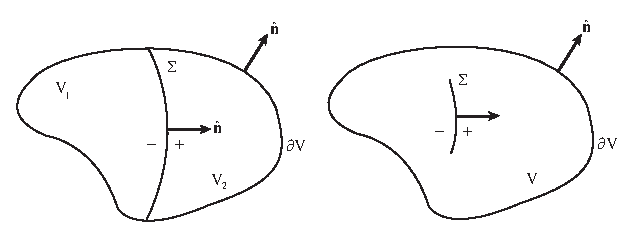
\includegraphics{../figures/appendixA/A1.eps}
\end{center}
\caption[extended Gauss]{\label{A.fig.Gauss}
({\em 左图\/})~包含两个相连区域~$V_1$~和~$V_2$~的复合积分区域,
两个相连区域被界面~$\Sigma$~隔开,界面两侧~
$\hat{\bf n}\cdot{\bf T}$~有一个不连续的跃变。
({\em 右图\/})~积分区域~$V$~中埋有定向表面~$\Sigma$,表面两侧~
$\hat{\bf n}\cdot{\bf T}$~有不连续跃变。
广义形式的高斯定理~(\ref{A.Gauss3})~适用于这两种情况。}
\end{figure}
在本书许多的应用中,上述结果导致在地球内部的各个内部界面处的跃变项~ $[\bnh\cdot\bT]^+_-=[\hat{n}_iT_{ij_1\cdots\,j_{q-1}}]^+_-$。当~$\Sigma$~ 是一个埋入~$V$~内的定向表面(例如断层)时,结果~(\ref{A.Gauss3})~ 仍然适用;这一结论很容易用极限推论来证明:在刺穿了一个“裂缝”~$V_{\varepsilon}$~的体积~$V-V_{\varepsilon}$~上积分,使“裂缝”逐渐塌缩到~$\Sigma$~的两侧上。

%\section{Surfaces}
\section{表面}

到目前为止,我们只关注了矢量和张量以及在三维欧式空间中作
用于它们的梯度和相关算子。
在定量全球地震学中也经常会遇到涉及在二维曲面上定义的矢量和张量的代数和微分运算。
在本节中,我们将讨论经典微分几何的基本概念,并将其用于这些运算。

%\subsection{Tangent vectors and tensors}
\subsection{切向矢量和张量}
\index{tangent vector|(}%
\index{tangent tensor|(}%
\index{vector!tangent|(}%
\index{tensor!tangent|(}%

在单位法向为~$\bnh$~的定向表面~$\Sigma$~上定义的任一矢量可以写成如下形式
\eq \label{A.tanvec}
\bu=\bnh u_n+\bu^{\Sigma},
\en
其中~$u_n=\bnh\cdot\bu$,$\bnh\cdot\bu^{\Sigma}=0$。
当然,$u_n$~当然是~$\bu$~的法向分量。任何具有~$\bnh\cdot\bu^{\Sigma}=0$~ 
性质的矢量~$\bu^{\Sigma}$~被称为{\em 切向矢量\/}。表达式~(\ref{A.tanvec})~将~$\bu$~ 分解为其法向和切向部分。任一二阶张量可以用类似但稍微复杂一些的方式
分解:
\eq \label{A.tanten}
\bT=\bnh\bnh T_{nn}+\bnh\bT^{n\Sigma}
+\bT^{\Sigma n}\bnh+\bT^{\Sigma\Sigma},
\en
其中$T_{nn}=\bnh\cdot\bT\cdot\bnh$。 
$\bT^{n\Sigma}$~和~$\bT^{\Sigma n}$~为满足~$\bnh\cdot\bT^{n\Sigma}
=\bnh\cdot\bT^{\Sigma n}=0$~的切向矢量,而~$\bT^{\Sigma\Sigma}$~是所谓的{\em 切向张量\/},以~$\bnh\cdot\bT^{\Sigma\Sigma}
=\bT^{\Sigma\Sigma}\cdot\bnh=\bzero$~定义。
$\bT$~的转置为
\eq
\bT^{\rm T}=\bnh\bnh T_{nn}+\bT^{n\Sigma}\bnh
+\bnh\bT^{\Sigma n}+(\bT^{\Sigma\Sigma})^{\rm T}.
\en
如果~$\bT$~是一个对称张量,则~$\bT^{\Sigma n}=\bT^{n\Sigma}$,
$(\bT^{\Sigma\Sigma})^{\rm T}=\bT^{\Sigma\Sigma}$。

两个矢量的点积为
\eq
\bu\cdot\bv=u_nv_n
+\bu^{\Sigma}\cdot\bv^{\Sigma},
\en
一个张量与一个矢量的左、右点积分别为
\eq
\bT\cdot\bu=\bnh(T_{nn}u_n
+\bT^{n\Sigma}\cdot\bu^{\Sigma})+\bT^{\Sigma n}u_n
+\bT^{\Sigma\Sigma}\cdot\bu^{\Sigma},
\en
\eq
\bu\cdot\bT=\bnh(u_nT_{nn}
+\bu^{\Sigma}\cdot\bT^{\Sigma n})+u_n\bT^{n\Sigma}
+\bu^{\Sigma}\cdot\bT^{\Sigma\Sigma}.
\en
显然,$\bT\cdot\bnh=\bnh T_{nn}+\bT^{\Sigma n}$,而~$\bnh\cdot\bT=\bnh T_{nn}+\bT^{n\Sigma}$。
\index{double dot product}%
最后,两个张量的双点积为
\eq
\bT\!:\!\bP=T_{nn}P_{nn}+\bT^{\Sigma n}\cdot\bP^{\Sigma n}
+\bT^{n\Sigma}\cdot\bP^{n\Sigma}+\bT^{\Sigma\Sigma}\!:\!
\bP^{\Sigma\Sigma}.
\en
切向张量最简单的的例子是{\em 表面单位张量\/}~$\bI^{\Sigma\Sigma}$,
\index{surface identity tensor}%
\index{identity tensor!surface}%
\index{tensor!surface identity}%
其定义为
\eq \label{A.metric}
\bI=\bnh\bnh+\bI^{\Sigma\Sigma}.
\en
该张量名副其实,因为对任何切向矢量~$\bu^{\Sigma}$~都有 $\bI^{\Sigma\Sigma}\cdot\bu^{\Sigma}=
\bu^{\Sigma}\cdot\bI^{\Sigma\Sigma}=\bu^{\Sigma}$。
很明显,表面单位张量是对称的:$(\bI^{\Sigma\Sigma})^{\rm T}=
\bI^{\Sigma\Sigma}$。
\index{tangent vector|)}%
\index{tangent tensor|)}%
\index{vector!tangent|)}%
\index{tensor!tangent|)}%

%\subsection{Surface gradient}
\subsection{表面梯度}
\index{surface gradient|(}%
\index{gradient!surface|(}%

三维梯度算子也可以分解为法向和切向部分:
\eq \label{A.surfgrad}
\bdel=\bnh\hspace{0.2 mm}\p_n+\bdel^{\Sigma},
\en
其中~$\p_n=\bnh\cdot\bdel$,$\bnh\cdot\bdel^{\Sigma}=0$。
切向部分~$\bdel^{\Sigma}$~被称为{\em 表面梯度\/}算子。由于~$\bdel^{\Sigma}$~只涉及
与表面~$\Sigma$~相切方向的微分,它可以作用于任何在~ $\Sigma$~上定义的标量、矢量或张量场,无论该场在表面以外是否也有定义。
正如~$\bdel\psi$~是标量场~$\psi$~在三维空间中变化最快方向上的变化率的一个度量,
标量场的表面梯度~$\bdel^{\Sigma}\psi$~也是~$\psi$~在~ $\Sigma$~上变化最快的切向方向上的变化率的一个度量。
在用算子~(\ref{A.surfgrad})~应用于如~(\ref{A.tanvec})--(\ref{A.tanten})~中的分解后的矢量和二阶张量时,
必须记住表面梯度也要作用于可变的单位法向矢量~$\bnh$;例如,一个矢量场的散度是 $\bdel\cdot\bu=(\p_n+
\bdel^{\Sigma}\cdot\bnh)u_n+\bdel^{\Sigma}\cdot\bu^{\Sigma}$,其中~ $\bdel^{\Sigma}\cdot\bnh={\rm tr}\,(\bdel^{\Sigma}\bnh)$。同样值得注意的是,
两个串连的算子~$\bdel^{\Sigma}\bdel^{\Sigma}$~并不是对称的;
事实上,很容易证明
\eq \label{A.surfgradsym}
[\bdel^{\Sigma}\bdel^{\Sigma}-\bnh\,(\bdel^{\Sigma}\bnh)
\cdot\bdel^{\Sigma}]^{\rm T}=\bdel^{\Sigma}\bdel^{\Sigma}
-\bnh\,(\bdel^{\Sigma}\bnh) \cdot\bdel^{\Sigma}.
\en
三维拉普拉斯算子~$\del^2=\bdel\cdot\bdel$~可以用法向导数~$\p_n$~和表面梯度~ $\bdel^{\Sigma}$~写为:
\eq \label{A.surfdelsq}
\del^2=\p_n^2+(\bdel^{\Sigma}\cdot\bnh)\p_n+(\del^{\Sigma})^2.
\en
用一个虽不标准但却显而易见的名称,我们将二维的标量微分算子
\eq \label{A.Beltrami}
(\del^{\Sigma})^2=\bdel^{\Sigma}\cdot\bdel^{\Sigma}=
{\rm tr}\,(\bdel^{\Sigma}\bdel^{\Sigma})
\en
称为{\em 表面拉普拉斯\/};
\index{surface Laplacian}%
\index{Laplacian!surface}%
在更专业的数学论述中,(\ref{A.Beltrami})~被称为{\em Beltrami算子\/}。
\index{Beltrami operator}%
\index{operator!Beltrami}%

如果~$\bv^{\Sigma}$~是一个定向曲面~$\Sigma$~上持续可微的切向矢量场,
{\em 二维广义高斯定理\/}表明
\index{Gauss' theorem!on a curved surface}%
\eq \label{A.2DGauss}
\int_{\Sigma}\bdel^{\Sigma}\cdot\bv^{\Sigma}\,d\/\Sigma=
\int_{\spar\Sigma}\hat{\bb}\cdot\bv^{\Sigma}\,dL.
\en
其中线积分是沿着曲面~$\Sigma$~的边界~$\p\Sigma$;
单位法向矢量~$\hat{\bb}$~与~$\Sigma$~相切且在~$\p\Sigma$~上指向~$\Sigma$~的外部。
对于二阶切向张量场~$\bT^{\Sigma\Sigma}$,有一个类似的结果,即
\eq \label{A.2DGauss2}
\int_{\Sigma}\bdel^{\Sigma}\cdot\bT^{\Sigma\Sigma}\,d\/\Sigma=
\int_{\spar\Sigma}\hat{\bb}\cdot\bT^{\Sigma\Sigma}\,dL.
\en
如果曲面~$\Sigma$~是封闭的,而封闭的表面是没有边界的,(\ref{A.2DGauss})~
和~(\ref{A.2DGauss2})~两式简化为
\eq \label{A.2DGauss3}
\int_{\Sigma}\bdel^{\Sigma}\cdot\bv^{\Sigma}\,d\/\Sigma=0,\qquad
\int_{\Sigma}\bdel^{\Sigma}\cdot\bT^{\Sigma\Sigma}\,d\/\Sigma=\bzero,
\en
%\index{surface gradient|)}%
%\index{gradient!surface|)}%

%\subsection{Covariance and contravariance}
\subsection{协变与逆变}
\index{covariance|(}%
\index{contravariance|(}%

令~$x^1$,$x^2$~为~$\Sigma$~上的二维(未必正交的)曲线坐标系统,
并以~$\p_{\alpha}$~表示对~$x^{\alpha}$~的普通偏导数(非协变导数)。
连接表面上坐标为~$x^1$、$x^2$~的点~$\br$~和坐标为~$x^1+dx^1$、 $x^2+dx^2$~的相邻点~$\br+d\/\br$~的微分切向矢量为
\eq \label{A.diffdist}
d\/\br=dx^{\alpha}(\p_{\alpha}\br).
\en
表面梯度算子~$\bdel^{\Sigma}$~和偏导数~$\p_{\alpha}$~之间的关系为
\eq \label{A.surfgrad2}
\bdel^{\Sigma}=(\bdel^{\Sigma}x^{\alpha})\p_{\alpha},\qquad
\p_{\alpha}=(\p_{\alpha}\br)\cdot\bdel^{\Sigma}.
\en
(\ref{A.diffdist})--(\ref{A.surfgrad2})~式及后续讨论中的希腊角标取值均为~1~和~2;任何
重复角标均意味着求和,且在上角标或下角标中只能出现一次。

$\bdel^{\Sigma}x^1$、$\bdel^{\Sigma}x^2$~
和~$\p_1\br$、$\p_2\br$~均可作为二维基,用来表示表面~ $\Sigma$~上的任意切向矢量和切向张量。
这两组基都不是正交归一的;但是,两者之间有关系
\eq \label{A.dual}
(\bdel^{\Sigma}x^{\alpha})\cdot(\p_{\beta}\br)
=\delta^{\alpha}_{\,\,\,\beta},\qquad
(\p_{\alpha}\br)\cdot(\bdel^{\Sigma}x^{\beta})
=\delta_{\alpha}^{\,\,\,\beta}.
\en
在这个意义上,它们互为{\em 对偶\/}基。
\index{dual basis}%
\index{basis!dual}%
$\delta^{\alpha}_{\,\,\,\beta}$~和~
$\delta_{\alpha}^{\,\,\,\beta}$~均表示二维克罗内克符号,当~$\alpha=\beta$~ 时,它等于~1,否则为~0;这里使用了两个独特但等同的符号,它们所遵循的约定是角标在上还是在下,以及角标的顺序都变得必须有所区分。我们把注意力局限在满足 
$\bnh\cdot(\p_1\br\times\p_2\br)>0$~
和~$\bnh\cdot(\bdel^{\Sigma}x^1
\times\bdel^{\Sigma}x^2)>0$~的右手曲线坐标系。

一个切向矢量~$\bu^{\Sigma}$~的{\em 协变分量\/}~$u_{\alpha}$
\index{component!covariant}%
\index{covariant component}%
和{\em 逆变分量\/}~$u^{\alpha}$
\index{component!contravariant}%
\index{contravariant component}%
的定义为
\eq
\bu^{\Sigma}=u_{\alpha}(\bdel^{\Sigma}x^{\alpha})
=u^{\alpha}(\p_{\alpha}\br).
\en
一个切向张量~$\bT^{\Sigma\Sigma}$~的协变分量~$T_{\alpha\beta}$、逆变分量~ $T^{\alpha\beta}$~以及两种{\em 混合分量\/}
\index{component!mixed}%
$T_{\alpha}^{\,\,\,\beta}$~
和~$T^{\alpha}_{\,\,\,\beta}$~可以同样地定义为
\eqa \lefteqn{
\bT^{\Sigma\Sigma}=T^{\alpha\beta}(\p_{\alpha}\br)(\p_{\beta}\br)
=T_{\alpha\beta}(\bdel^{\Sigma}x^{\alpha})(\bdel^{\Sigma}x^{\beta})}
\nonumber \\
&&\mbox{}=T^{\alpha}_{\,\,\,\beta}(\p_{\alpha}\br)(\bdel^{\Sigma}x^{\beta})
=T_{\alpha}^{\,\,\,\beta}(\bdel^{\Sigma}x^{\alpha})(\p_{\beta}\br).
\ena
要得到一个给定矢量~$\bu^{\Sigma}$~或张量~$\bT^{\Sigma\Sigma}$~的分量,
我们用对偶基与其点乘,并利用~(\ref{A.dual})~式,得到
\eq \label{A.vecocon}
u_{\alpha}=(\p_{\alpha}\br)\cdot\bu^{\Sigma},\qquad
u^{\alpha}=(\bdel^{\Sigma}x^{\alpha})\cdot\bu^{\Sigma}
\en
和
\eq
T_{\alpha\beta}=(\p_{\alpha}\br)\cdot
\bT^{\Sigma\Sigma}\cdot(\p_{\beta}\br),
\en
\eq
T^{\alpha\beta}=(\bdel^{\Sigma}x^{\alpha})\cdot
\bT^{\Sigma\Sigma}\cdot(\bdel^{\Sigma}x^{\beta}),
\en
\eq
T_{\alpha}^{\,\,\,\beta}=(\p_{\alpha}\br)\cdot
\bT^{\Sigma\Sigma}\cdot(\bdel^{\Sigma}x^{\beta}),
\en
\eq
T^{\alpha}_{\,\,\,\beta}=(\bdel^{\Sigma}x^{\alpha})\cdot
\bT^{\Sigma\Sigma}\cdot(\p_{\beta}\br).
\en
每个投币口都为切向的更高阶张量的协变、逆变和混合分量可以用类似的方式定义。
\index{covariance|)}%
\index{contravariance|)}%

%\subsection{Metric tensor}
\subsection{度量张量}
\index{metric tensor|(}%
\index{tensor!metric|(}%

由于历史原因,表面单位张量~$\bI^{\Sigma\Sigma}$~的分量通常写为
\eq
g_{\alpha\beta}=(\p_{\alpha}\br)\cdot(\p_{\beta}\br),\qquad
g^{\alpha\beta}=(\bdel^{\Sigma}x^{\alpha})\cdot(\bdel^{\Sigma}x^{\beta}),
\en
\eq
g_{\alpha}^{\,\,\,\beta}=(\p_{\alpha}\br)\cdot(\bdel^{\Sigma}x^{\beta}),\qquad
g^{\alpha}_{\,\,\,\beta}=(\bdel^{\Sigma}x^{\alpha})\cdot(\p_{\beta}\br).
\en
对偶关系~(\ref{A.dual})~意味着~$g_{\alpha}^{\,\,\,\beta}
=\delta_{\alpha}^{\,\,\,\beta}$~和~$g^{\alpha}_{\,\,\,\beta}
=\delta^{\alpha}_{\,\,\,\beta}$;因此
\eq \label{A.ISIGMA}
\bI^{\Sigma\Sigma}=(\p_{\alpha}\br)(\bdel^{\Sigma}x^{\beta})
=(\bdel^{\Sigma}x^{\alpha})(\p_{\beta}\br)=\bdel^{\Sigma}\br.
\en
(\ref{A.ISIGMA})~式的缩并为
\eq \label{A.ISIGMATR}
{\rm tr}\,\bI^{\Sigma\Sigma}=\bdel^{\Sigma}\cdot\br=2.
\en
(\ref{A.ISIGMA})~和~(\ref{A.ISIGMATR})~这两个结果推广了熟知的三维空间等式~ $\bI=\bdel\br$~和~${\rm tr}\,\bI=\bdel\cdot\br=3$。

将~(\ref{A.vecocon})~式用于两种基矢量场~$\p_{\alpha}\br$~和~$\bdel^{\Sigma}x^{\alpha}$~后,我们发现
\eq \label{A.ginverse}
\p_{\alpha}\br=g_{\alpha\beta}(\bdel^{\Sigma}x^{\beta}),\qquad
\bdel^{\Sigma}x^{\alpha}=g^{\alpha\beta}(\p_{\beta}\br).
\en
(\ref{A.ginverse})式表明,对称的协变和逆变分量矩阵$g_{\alpha\beta}$
和$g^{\alpha\beta}$互为彼此的逆:
\eq
g_{\alpha\gamma}g^{\gamma\beta}=g_{\alpha}^{\,\,\,\beta},\qquad
g^{\alpha\gamma}g_{\gamma\beta}=g^{\alpha}_{\,\,\,\beta}.
\en
这是角标升降规则的一个特例,
\index{index!lowering and raising of}%
它可以用来将一个切向矢量~$\bu^{\Sigma}$~的逆变分量转换为协变量,反之亦然:
\eq
u_{\alpha}=g_{\alpha\beta}u^{\beta},\qquad
u^{\alpha}=g^{\alpha\beta}u_{\beta}
\en
也可以用于切向张量~$\bT^{\Sigma\Sigma}$:
\eq
T_{\alpha\beta}=g_{\alpha\gamma}T^{\gamma}_{\,\,\,\beta}
=g_{\alpha\gamma}g_{\beta\eta}T^{\gamma\eta},\qquad\!\!
T^{\alpha\beta}=g^{\alpha\gamma}T_{\gamma}^{\,\,\,\beta}
=g^{\alpha\gamma}g^{\beta\eta}T_{\gamma\eta}
\en
两个切向矢量的点积可以写成下面任何一种等价形式
\eq
\bu^{\Sigma}\cdot\bv^{\Sigma}=u_{\alpha}v^{\alpha}
=u^{\alpha}v_{\alpha}=g_{\alpha\beta}u^{\alpha}v^{\beta}
=g^{\alpha\beta}u_{\alpha}v_{\beta}.
\en
利用角标符号升降规则,涉及更高阶切向张量的点积同样可以用
张量的协变、逆变或混合分量来表达。
一个切向矢量的{\em 表面散度\/}为
\index{surface divergence}%
\index{divergence!surface}%
\eq \label{A.divneed16}
\bdel^{\Sigma}\cdot\bu^{\Sigma}=\half g^{\alpha\beta}
\partial_\gamma(g_{\alpha\beta}u^\gamma).
\en
(\ref{A.ISIGMATR})~式以希腊角标形式可以表示为~$g^{\alpha\beta}g_{\alpha\beta}=g^{\alpha}_{\,\,\,\alpha}=2$。

曲面~$\Sigma$~上坐标为~$x^1$、$x^2$~的点~$\br$~和坐标为~$x^1+dx^1$、
$x^2+dx^2$~的相邻点~$\br+d\/\br$~之间的距离平方~$ds^2$~为
\eq \label{A.dist}
ds^2=d\/\br\cdot d\/\br=g_{\alpha\beta}\,dx^{\alpha}dx^{\beta}.
\en
(\ref{A.dist})~式表明表面单位张量~$\bI^{\Sigma\Sigma}$~ 
是~$\Sigma$~上的{\em 度量张量\/}。
$g_{\alpha\beta}\,dx^{\alpha}dx^{\beta}$~这一微分-几何表达式被称为{\em 第一基本形式\/}。
\index{first fundamental form}%
\index{fundamental form!first}%
\index{metric tensor|)}%
\index{tensor!metric|)}%

%\subsection{Curvature tensor}
\subsection{曲率张量}
\index{curvature tensor|(}%
\index{tensor!curvature|(}%

传统上用来衡量表面~$\Sigma$~的曲率是借由如下的量
\eq \label{A.Fdef}
\bF^{\Sigma\Sigma}=(\bdel^{\Sigma}\bI^{\Sigma\Sigma})\cdot\bnh
=(\bdel^{\Sigma}\bdel^{\Sigma}\br)\cdot\bnh.
\en
从定义~(\ref{A.Fdef})~可以明显看出~$\bF^{\Sigma\Sigma}$~ 是一个对称切向张量;即~$\bnh\cdot\bF^{\Sigma\Sigma}=
\bF^{\Sigma\Sigma}\cdot\bnh=\bzero$~和
$(\bF^{\Sigma\Sigma})^{\rm T}=\bF^{\Sigma\Sigma}$。
从坐标为~$x^1+dx^1$、$x^2+dx^2$~的点~$\br+d\/\br$~到在~$\Sigma$~上坐标为~$x^1$, $x^2$~的点~$\br$~并与~$\Sigma$~相切的平面的垂直距离~$dn$~为
\eq \label{A.perpdist}
dn=\half (d\/\br\cdot\bF^{\Sigma\Sigma}\cdot d\/\br)=
\half f_{\alpha\beta}\,dx^{\alpha}dx^{\beta},
\en
其中~$f_{\alpha\beta}=(\p_{\alpha}\br)\cdot\bF^{\Sigma\Sigma}
\cdot(\p_{\beta}\br)$~为~$\bF^{\Sigma\Sigma}$~的协变分量。与单位法向矢量~ $\bnh$~方向相同的微分距离~$dn$~为正。
由于相切平面的几何构建明确认定表面~$\Sigma$~是掩埋在
三维欧氏空间中的,因此~$\bF^{\Sigma\Sigma}$~被称为“外”{\em 曲率张量\/}。
二次表达式~$\half f_{\alpha\beta}dx^{\alpha}dx^{\beta}$~被称为{\em 第二基本形式\/}。
\index{second fundamental form}%
\index{fundamental form!second}%

取~$\bI^{\Sigma\Sigma}\cdot\bnh=(\bdel^{\Sigma}\br)\cdot\bnh=\bzero$~的表面梯度,我们得到曲率张量的另一个表达式:
\eq \label{A.Fdef2}
\bF^{\Sigma\Sigma}=-\bdel^{\Sigma}\bnh.
\en
$\bF^{\Sigma\Sigma}$~的对称性意味着
\eq \label{A.Fsymm}
(\bdel^{\Sigma}\bnh)^{\rm T}=\bdel^{\Sigma}\bnh.
\en
单位法向矢量的散度为
\eq \label{A.delSign}
\bdel^{\Sigma}\cdot\bnh=\frac{1}{R_1}+\frac{1}{R_2},
\en
其中~$1/R_1$~和~$1/R_2$~是~$\Sigma$~在~$\br$~点处的两个{\em 主曲率\/}。
\index{principal curvature}%
\index{curvature!principal}%
在这一背景下,最后一个有用的关系式为~$\bdel^{\Sigma}\bI^{\Sigma\Sigma}
=-\bdel^{\Sigma}(\bnh\bnh)$。
\index{curvature tensor|)}%
\index{tensor!curvature|)}%

%\section{Spherical Polar Coordinates}
\section{球极坐标}
\index{spherical polar coordinates|(}%
\label{A.sec.polcoord}

令~$r=\|\br\|$~为从原点到点~$\br=x\bxh+y\byh+z\bzh$~的径向距离,
$0\leq \theta\leq\pi$~为极轴或~$\bzh$~轴与~$\br$~的夹角, 
$0\leq \phi\leq 2\pi$~为~$\bxh$~轴与~$\br$~在赤道上的投影~$x\bxh+y\byh$~之间的夹角。
任意点~$\br$~都可以用这些{\em 球极坐标\/}来唯一地定义;角度~$\theta$~和~$\phi$~ 分别为地心{\em 余维度\/}和{\em 经度\/}。
\index{colatitude}%
\index{longitude}%
点~$\br$~的笛卡尔坐标~$x$、$y$、$z$~与其球极坐标~$r$、$\theta$、$\phi$~之间的关系为
\eq \label{A.xyzrtp}
x=r\sin\theta\cos\phi,\qquad y=r\sin\theta\sin\phi,\qquad z=r\cos\theta.
\en
反之,以~$x$、$y$、$z$~表示~$r$、$\theta$、$\phi$~的关系式为
\begin{displaymath}
r=\sqrt{x^2+y^2+z^2},\qquad\theta=\arctan(\sqrt{x^2+y^2}/z),
\end{displaymath}
\eq
\qquad\qquad\qquad\phi=\arctan(y/x).
\en
单位矢量~$\brh$、$\bthetah$、$\bphih$~的方向分别为~$r$、$\theta$、$\phi$~增加的方向,它们组成一个局部的右手正交归一基,且与笛卡尔坐标系的基~$\bxh$、$\byh$、$\bzh$~存在以下关系
\eq \label{A.needinC}
\brh=\bxh\sin\theta\cos\phi+\byh\sin\theta\sin\phi
+\bzh\cos\theta,
\en
\eq \label{A.need1}
\bthetah=\bxh\cos\theta\cos\phi+\byh\cos\theta\sin\phi
-\bzh\sin\theta,
\en
\eq \label{A.need2}
\bphih=-\bxh\sin\phi+\byh\cos\phi.
\en
反之,
\eq
\bxh=\brh\sin\theta\cos\phi+\bthetah\cos\theta\cos\phi
-\bphih\sin\phi,
\en
\eq
\byh=\brh\sin\theta\sin\phi+\bthetah\cos\theta\sin\phi
+\bphih\cos\phi,
\en
\eq
\bzh=\brh\cos\theta-\bthetah\sin\theta.
\en
矢量~$\brh$、$\bthetah$、$\bphih$~的偏导数为
\eq
\p_r\brh=\bzero,\qquad
\p_{\theta}\brh=\bthetah,\qquad
\p_{\phi}\brh=\bphih\sin\theta,
\en
\eq
\p_r\bthetah=
\bzero,\qquad
\p_{\theta}\bthetah=-\brh,\qquad
\p_{\phi}\bthetah=\bphih\cos\theta,
\en
\eq
\p_r\bphih=\bzero,\qquad
\p_{\theta}\bphih=\bzero,\qquad
\p_{\phi}\bphih=-\brh\sin\theta-\bthetah\cos\theta.
\en
三维单位张量可以写成两种等价形式中的任何一种:$\bI=\bxh\bxh
+\byh\byh+\bzh\bzh=\brh\brh+\bthetah\bthetah+\bphih\bphih$。
\index{spherical polar coordinates|)}%

%\subsection{Unit sphere}
\subsection{单位球体}
\index{unit sphere|(}%

我们可以方便地将~$\theta$、$\phi$~视为{\em 单位球\/}上的曲线坐标;
我们用~$\Omega$~来表示这个由所有~$\|\brh\|=1$~的点组成的球体。三维梯度算子~ $\bdel=\bxh\p_x+\byh\p_y+\bzh\p_z$~可以用偏导数~$\p_r$、$\p_{\theta}$、$\p_{\phi}$~表示为
\eq \label{A.del1def}
\bdel=\brh\p_r+r^{-1}\bdel_1,
\en
其中
\eq \label{A.del1def2}
\bdel_1=\bthetah\p_{\theta}+\bphih(\sin\theta)^{-1}\p_{\phi}.
\en
算子~$\bdel_1$~是单位球上的无量纲表面梯度。
\index{surface gradient!on the unit sphere}%
$\Omega$~上三个单位矢量~$\brh$、$\bthetah$、$\bphih$~的表面梯度为
\eq \label{A.del1rhat}
\bdel_1\brh=\bthetah\bthetah+\bphih\bphih,
\en
\eq
\bdel_1\bthetah=-\bthetah\brh+\bphih\bphih\cot\theta,
\en
\eq \label{A.del1phat}
\bdel_1\bphih=-\bphih\brh-\bphih\bthetah\cot\theta.
\en
取~(\ref{A.del1rhat})--(\ref{A.del1phat})~三式的迹,我们得到
\eq \label{A.div1hats}
\bdel_1\cdot\brh=2,\qquad
\bdel_1\cdot\bthetah=\cot\theta,\qquad
\bdel_1\cdot\bphih=0.
\en
应用楔形算子~$\wedge$~可以得到类似的关系式
\eq \label{A.curl1hats}
\bdel_1\times\brh=\bzero,\qquad
\bdel_1\times\bthetah=\bphih,\qquad
\bdel_1\times\bphih=-\bthetah+\brh\cot\theta.
\en
正如预期的,(\ref{A.div1hats})~中的第一个公式与~(\ref{A.ISIGMATR})~和~(\ref{A.delSign})~中的一般法则是相符的。

由于~$\br\times\bdel=\brh\times\bdel_1$,算子 $\br\times\bdel=\bxh(y\p_z-z\p_y)+\byh(z\p_x-x\p_z)
+\bzh(x\p_z-z\p_x)$~也可被认为是作用在单位球上。
无量纲叉乘积~$\brh\times\bdel_1$~的球极坐标表达式为
\eq \label{A.surfcurl}
\brh\times\bdel_1=-\bthetah(\sin\theta)^{-1}\p_\phi+\bphih\,\p_\theta.
\en
正如点积~$d\/\br\cdot\bdel_1\psi$~是标量场~$\psi$~在具有无穷小位移点\/ $\brh+d\/\brh$~处的变化的一个度量,标量三重积~$d\/\bomega\cdot\brh\times\bdel_1\psi$~可以被视为标量场~$\psi$~在具有无穷小旋转点~$\brh+d\/\bomega\times\brh$~处的变化的一个度量:
\eq
\psi(\brh+d\/\brh)=\psi(\brh)+d\/\brh\cdot\bdel_1\psi(\brh)+\cdots,
\en
\eq \label{A.diffrot}
\psi(\brh+d\/\bomega\times\brh)=\psi(\brh)+
d\/\bomega\cdot\brh\times\bdel_1\psi(\brh)+\cdots.
\en
我们将无量纲算子~~$\brh\times\bdel_1$称为表面旋度。
\index{surface curl}%
\index{curl!on the unit sphere}%
在~(\ref{A.diffrot})~式中与旋转矢量~$d\/\bomega$~点乘的部分
可以写成任一等价的形式~$\brh\times\bdel_1\psi=\br\times\bdel\psi
=-\bdel\times(\br\psi)=-\bdel_1\times(\brh\psi)$。在附录~B.12~中,我们会看到~$\bdel_1$~和~$\brh\times\bdel_1$~这两个算子在用标量表达~$\Omega$~上的切向矢量场中扮演了平行的角色。

表面梯度~$\bdel_1$~和旋度~$\brh\times\bdel_1$~的重复应用产生更高阶的张量算子,其中前四个是
\eqa \label{A.del1del1}
\lefteqn{\bdel_1\bdel_1=-\bthetah\brh\,\p_{\theta}-\bphih\brh\,
(\sin\theta)^{-1}\p_{\phi}+\bthetah\bthetah\,\p_{\theta}^2} \nonumber \\
&&\mbox{}+(\bthetah\bphih+\bphih\bthetah)(\sin\theta)^{-1}
(\p_\theta\p_\phi-\cot\theta\,\p_\phi) \nonumber \\
&&\mbox{}+\bphih\bphih\,[(\sin\theta)^{-2}\p_\phi^2+\cot\theta\,\p_\theta],
\ena
\eqa \label{A.del1rdel1}
\lefteqn{\bdel_1(\brh\times\bdel_1)=\bthetah\brh\,(\sin\theta)^{-1}\p_{\phi}
-\bphih\brh\,\p_{\theta}} \nonumber \\
&&\mbox{}-(\bthetah\bthetah-\bphih\bphih)(\sin\theta)^{-1}
(\p_\theta\p_\phi-\cot\theta\,\p_\phi) \nonumber \\
&&\mbox{}+\bthetah\bphih\,\p_\theta^2-\bphih\bthetah
\,[(\sin\theta)^{-2}\p_\phi^2+\cot\theta\,\p_{\theta}],
\ena
\eqa \label{A.rdel1del1}
\lefteqn{(\brh\times\bdel_1)\bdel_1=\bthetah\brh\,(\sin\theta)^{-1}\p_{\phi}
-\bphih\brh\,\p_{\theta}} \nonumber \\
&&\mbox{}-(\bthetah\bthetah-\bphih\bphih)(\sin\theta)^{-1}
(\p_\theta\p_\phi-\cot\theta\,\p_\phi) \nonumber \\
&&\mbox{}-\bthetah\bphih\,[(\sin\theta)^{-2}\p_\phi^2
+\cot\theta\,\p_{\theta}]+\bphih\bthetah\,\p_\theta^2,
\ena
\eqa \label{A.rdel1rdel1}
\lefteqn{(\brh\times\bdel_1)(\brh\times\bdel_1)
=\bthetah\brh\,\p_{\theta}+\bphih\brh\,(\sin\theta)^{-1}\p_{\phi}} \nonumber \\
&&\mbox{}+\bthetah\bthetah\,[(\sin\theta)^{-2}\p_\phi^2+\cot\theta\,\p_\theta]
+\bphih\bphih\,\p_{\theta}^2 \nonumber \\
&&\mbox{}-(\bthetah\bphih+\bphih\bthetah)(\sin\theta)^{-1}
(\p_\theta\p_\phi-\cot\theta\,\p_\phi).
\ena
无量纲双重梯度~$\bdel_1\bdel_1$~和无量纲双重旋度~ $(\brh\times\bdel_1)(\brh\times\bdel_1)$~都是不对称的;事实上,
\eq \label{A.del1del1T}
(\bdel_1\bdel_1-\brh\bdel_1)^{\rm T}=\bdel_1\bdel_1-\brh\bdel_1,
\en
\vspace*{-2.0mm}
\eqa \label{A.rdelr1del1T}
\lefteqn{[(\brh\times\bdel_1)(\brh\times\bdel_1)
-(\brh\bdel_1)^{\rm T}]^{\rm T}} \nonumber \\
&&\mbox{}=(\brh\times\bdel_1)(\brh\times\bdel_1)-(\brh\bdel_1)^{\rm T},
\ena
\eq \label{A.del1rdel1T}
[\bdel_1(\brh\times\bdel_1)-\brh(\brh\times\bdel_1)]^{\rm T}=
(\brh\times\bdel_1)\bdel_1-\brh(\brh\times\bdel_1).
\en
(\ref{A.del1del1T})~是一般曲面~$\Sigma$~上的对称关系~(\ref{A.surfgradsym})~的一个特例。

三维拉普拉斯算子~$\del^2=\bdel\cdot\bdel$~的球坐标表达式为
\eq
\del^2=\p_r^2+2r^{-1}\p_r+r^{-2}\del_1^2.
\en
(\ref{A.del1del1})~和~(\ref{A.rdel1rdel1})~两式的缩并均可以得到{\em 表面拉普拉斯\/}算子~$\del_1^2=\bdel_1\cdot\bdel_1
=(\brh\times\bdel_1)\cdot(\brh\times\bdel_1)$
\index{surface Laplacian}%
\index{Laplacian!surface}%
\eq
\del_1^2=\p_\theta^2+\cot\theta\,\p_\theta+(\sin\theta)^{-2}\p_\phi^2.
\en
(\ref{A.del1rdel1})~和~(\ref{A.rdel1del1})~两式的缩并证实无量纲梯度和旋度处处正
交:$\bdel_1\cdot(\brh\times\bdel_1)=(\brh\times\bdel_1)\cdot\bdel_1=0$。
最后,我们注意到~$\bdel_1\times\bdel_1=-(\brh\times\bdel_1)
\times(\brh\times\bdel_1)=\brh\times\bdel_1$,而~$\bdel_1\times(\brh\times\bdel_1)=-(\brh\times\bdel_1)\times\bdel_1
=\brh\,\del_1^2-\bdel_1$。

$\Omega$~上的表面单位张量~$\bI^{\Omega\Omega}=\bI-\brh\brh=\bthetah\bthetah+\bphih\bphih$~的协变和逆变分量为~
$g_{11}=1$、$g_{12}=g_{21}=0$、$g_{22}=\sin^2\theta$~
和~$g^{11}=1$、$g^{12}=g^{21}=0$、$g^{22}=(\sin\theta)^{-2}$,这里我们
设定~$x^1=\theta$~和~$x^2=\phi$。我们可以利用这些结果来定义和整理切向矢量~ $\bu^{\Omega}$~的协变分量~$u_{\alpha}$~和逆变分量~$u^{\alpha}$,以及切向张量~ $\bT^{\Omega\Omega}$~的协变分量~$T_{\alpha\beta}$、逆变分量~$T^{\alpha\beta}$~与混合分量~$T_{\alpha}^{\,\,\,\beta}$~和~$T^{\alpha}_{\,\,\,\beta}$;
然而,正如我们接下来要讨论的,用“普通的”或{\em 物理球极分量\/}来进行运算在物理上更具吸引力,而数学上也不会更费力气。
\index{unit sphere|)}%

%\subsection{Physical components}
\subsection{物理分量}
\index{physical components|(}%
\index{component!physical|(}%

三维矢量场可以写成以下形式
\eq \label{A.vecrtp}
\bu=u_r\brh+u_{\theta}\bthetah+u_{\phi}\bphih,
\en
其中~$u_r=\brh\cdot\bu$, $u_{\theta}=\bthetah\cdot\bu$~
和~$u_{\phi}=\bphih\cdot\bu$。二阶张量场的相应表达式为
\eqa \label{A.tenrtp} \lefteqn{
\bT=T_{rr}\brh\brh+T_{r\theta}\brh\bthetah+T_{r\phi}\brh\bphih} \nonumber \\
&&\mbox{}\qquad
+T_{\theta r}\bthetah\brh+T_{\theta\theta}\bthetah\bthetah+
T_{\theta\phi}\bthetah\bphih
\nonumber \\
&&\mbox{}\qquad\qquad
+T_{\phi r}\bphih\brh+T_{\phi\theta}\bphih\bthetah+T_{\phi\phi}\bphih\bphih,
\ena
其中~$T_{rr}=\brh\cdot\bT\cdot\brh$、
$T_{r\theta}=\brh\cdot\bT\cdot\bthetah,
\ldots,T_{\phi\phi}=\bphih\cdot\bT\cdot\bphih$。一般而言,当
我们在本书中用球极坐标写出如~$u_{\phi}$~或~$T_{\phi\phi}$~这样的表达式时,
我们指的是~(\ref{A.vecrtp})~和~(\ref{A.tenrtp})~式中所示的~$\bu$~和~$\bT$~的物理分量,
而并非其相应的协变分量~$\sin\theta\,u_{\phi}$~和~$\sin^2\theta\,T_{\phi\phi}$。 
利用局部基矢量~$\brh$、$\bthetah$、$\bphih$~的正交归一性,
矢量和张量积可以很容易地用物理分量来计算。
例如,两个矢量~$\bu$~和~$\bv$~的点积是 $\bu\cdot\bv=u_rv_r+u_{\theta}v_{\theta}+u_{\phi}v_{\phi}$。
\vspace{-0.4 mm},而叉乘积则为~$\bu\times\bv=\brh(u_{\theta}v_{\phi}
-u_{\phi}v_{\theta})+\bthetah(u_{\phi}v_r-u_rv_{\phi})
+\bphih(u_rv_{\theta}-u_{\theta}v_r)$。两个张量的双重点积为~ $\bT\!:\!\bP=T_{rr}P_{rr}+T_{r\theta}P_{\theta r}
+\cdots+T_{\phi\phi}P_{\phi\phi}$。

三维导数可以利用分解公式~(\ref{A.del1def})--(\ref{A.del1def2})~和微分基矢量关系~(\ref{A.del1rhat})--(\ref{A.del1phat})~
直接计算。矢量场~$\bdel\bu$~的梯度
\index{gradient!of a vector field}%
及其对应的对称张量~$\beps=\half[\bdel\bu+(\bdel\bu)^{\rm T}]$~可以写为
\eqa \label{A.Jeroen1}
\lefteqn{\bdel\bu=(\p_ru_r)\brh\brh+r^{-1}(\p_\theta u_\theta+u_r)
\bthetah\bthetah} \nonumber \\
&&\mbox{}
+r^{-1}[(\sin\theta)^{-1}\p_\phi u_\phi+u_r+u_\theta\cot\theta]
\bphih\bphih \nonumber \\
&&\mbox{}
+(\p_ru_\theta)\brh\bthetah+r^{-1}(\p_\theta u_r-u_\theta)\bthetah\brh
\nonumber \\
&&\mbox{}+(\p_ru_\phi)\brh\bphih
+r^{-1}[(\sin\theta)^{-1}\p_\phi u_r-u_\phi]\bphih\brh
\nonumber \\
&&\mbox{}+r^{-1}(\p_\theta u_\phi)\,\bthetah\bphih
+r^{-1}[(\sin\theta)^{-1}\p_\phi u_\theta-u_\phi\cot\theta]\bphih\bthetah
\ena
和
\eqa \label{A.Jeroen2}
\lefteqn{\beps
=(\p_ru_r)\brh\brh+r^{-1}(\p_\theta u_\theta+u_r)\bthetah\bthetah} \nonumber \\
&&\mbox{}+r^{-1}[(\sin\theta)^{-1}\p_\phi u_\phi+u_r+u_\theta\cot\theta]
\bphih\bphih\nonumber \\
&&\mbox{}
+\half[\p_ru_\theta+r^{-1}(\p_\theta u_r-u_\theta)]
(\brh\bthetah+\bthetah\brh)\nonumber \\
&&\mbox{}
+\half\{\p_ru_\phi+r^{-1}[(\sin\theta)^{-1}\p_\phi u_r
-u_\phi]\}(\brh\bphih+\bphih\brh) \nonumber \\
&&\mbox{}+\half r^{-1}[\p_\theta u_\phi+(\sin\theta)^{-1}
\p_\phi u_\theta-u_\phi\cot\theta]
(\bthetah\bphih+\textcolor{red}{\bphih\bthetah}).
\ena
\index{divergence!of a vector field}%
(\ref{A.Jeroen1})~或~(\ref{A.Jeroen2})~的缩并所得到的散度~$\bdel\cdot\bu={\rm tr}\,\beps$~为
\eqa \label{A.divergence2} \lefteqn{
\bdel\cdot\bu=\p_ru_r} \nonumber \\
&&\mbox{}+r^{-1}[\textcolor{green}{2 u_r} + 
\p_\theta u_\theta+u_\theta\cot\theta
+(\sin\theta)^{-1}\p_\phi u_\phi].
\ena
(\ref{A.divergence2})~中括号内的表达式是表面散度:
\index{surface divergence}%
\index{divergence!surface}%
\eq
\bdel_1\cdot\bu=\textcolor{red}{2u_r}+\p_\theta u_\theta+u_\theta\cot\theta
+(\sin\theta)^{-1}\p_\phi u_\phi.
\en
一个矢量场的旋度~$\bdel\times\bu$~为
\index{curl!of a vector field}%
\eqa
\lefteqn{\bdel\times\bu=r^{-1}[\p_\theta u_\phi+u_\phi\cot\theta
-(\sin\theta)^{-1}\p_\phi u_\theta]\brh} \nonumber \\
&&\mbox{}+[r^{-1}(\sin\theta)^{-1}\p_\phi u_r-\p_ru_\phi
-r^{-1}u_\phi]\bthetah \nonumber \\
&&\mbox{}+(\p_ru_\theta+r^{-1}u_\theta-r^{-1}\p_\theta u_r)\bphih
\ena
而拉普拉斯算子~
$\del^2\bu=\bdel(\bdel\cdot\bu)-\bdel\times(\bdel\times\bu)$~是
\index{Laplacian!of a vector field}%
\eqa \label{A.del2bu}
\lefteqn{\del^2\bu=\{[\p_r^2+2r^{-1}\p_r+r^{-2}
(\p_{\theta}^2+\cot\theta\,\p_{\theta}+(\sin\theta)^{-2}
\p_{\phi}^2)]u_r} \nonumber \\
&&\mbox{}-2r^{-2}[u_r+
\p_\theta u_\theta+u_\theta\cot\theta
+(\sin\theta)^{-1}\p_\phi u_\phi]\}\,\brh \nonumber \\
&&\mbox{}+\{[\p_r^2+2r^{-1}\p_r+r^{-2}
(\p_{\theta}^2+\cot\theta\,\p_{\theta}+(\sin\theta)^{-2}
\p_{\phi}^2)]u_\theta \nonumber \\
&&\mbox{}+r^{-2}[2\p_\theta u_r-(\sin\theta)^{-2}u_\theta
-2(\sin\theta)^{-1}\cot\theta\,\p_\phi u_\phi]\}\,\bthetah \nonumber \\
&&\mbox{}+\{[\p_r^2+2r^{-1}\p_r+r^{-2}
(\p_{\theta}^2+\cot\theta\,\p_{\theta}+(\sin\theta)^{-2}
\p_{\phi}^2)]u_\phi \nonumber \\
&&\mbox{}+r^{-2}(\sin\theta)^{-1}[2\p_\phi u_r
+2\cot\theta\,\p_\phi u_\theta-(\sin\theta)^{-1}u_\phi]\}\,\bphih.
\ena
(\ref{A.del2bu})~式中第一、第三和第五行分别为标量拉普拉斯算子~$\del^2u_r$、 $\del^2u_{\theta}$~和~
$\del^2u_{\phi}$。最后,二阶张量场的散度~$\bdel\cdot\bT$~为
\index{divergence!of a tensor field}%
\eqa \label{A.LAST}
\lefteqn{\bdel\cdot\bT=\{\p_rT_{rr}+r^{-1}[\p_\theta T_{\theta r}
+(\sin\theta)^{-1}\p_\phi T_{\phi r}} \nonumber \\
&&\mbox{}+2T_{rr}-T_{\theta\theta}-T_{\phi\phi}
+\cot\theta \,T_{\theta r}]\}\,\brh \nonumber \\
&&\mbox{}+\{\p_rT_{r\theta}+r^{-1}[\p_\theta T_{\theta\theta}
+(\sin\theta)^{-1}\p_\phi T_{\phi\theta} \nonumber \\
&&\mbox{}+2T_{r\theta}+T_{\theta r}
+\cot\theta(T_{\theta\theta}-T_{\phi\phi})]\}\,\bthetah \nonumber \\
&&\mbox{}+\{\p_rT_{r\phi}+r^{-1}[\p_\theta T_{\theta\phi}
+(\sin\theta)^{-1}\p_\phi T_{\phi\phi} \nonumber \\
&&\mbox{}+2T_{r\phi}+T_{\phi r}
+\cot\theta(T_{\theta\phi}+T_{\phi\theta})]\}\,\bphih.
\ena
上述表达式十分冗长,而~$\bdel(\bdel\cdot\bu)$~
和~$\bdel\times(\bdel\times\bu)$~则让人更难忍受,这为我们在附录~B~和~C~中介绍的~$\bu$~和~$\bT$~的另外的表达方式提供了足够的理由。
\index{physical components|)}%
\index{component!physical|)}%
